\chapter{Integration}
%\todo{Remove COmment!!!!}
%\begin{comment}

\begin{enumerate}[\indent I)]
\item \begin{enumerate}[a)]
\item Gegeben sei eine stetige Funktion $f : \lbrack a,b\rbrack \rightarrow \mathbb{R}$. Gesucht ist eine differenzierbare Funktion $F: \lbrack a,b\rbrack \rightarrow \mathbb{R}$ mit $$F'(t)=f(t), \forall t \in \lbrack a,b \rbrack$$
\item Für Naturwissenschaft und Technik ist die folgende Verallgemeinerung von a) wichtig:\\
Sei $f:\lbrack a,b\rbrack \times \mathbb{R} \rightarrow \mathbb{R}$ gegeben. Gesucht ist eine differenzierbare Funktion $\varphi : \lbrack a,b\rbrack \rightarrow \mathbb{R}$ mit $$\varphi ' (t)=f(t,\varphi (t)), t\in \lbrack a,b \rbrack$$ Man nennt ein solches $\varphi$ eine Lösung der Differentialgleichung $$y'=f(x,y)$$
\end{enumerate}
\item Viele in der Natur und Ingenieurwissenschaften auftretenden Grössen benötigen zu ihrer exakten Definition einen Grenzprozess der Folgenden art: \\
Wirkt eine konstante Kraft f längs eines Weges der Länge $s$, und zwar längs der $x$-Achse vom Punkt $a$ bis zum Punkt $b:=a+s$, so versteht man unter der von der konstanten Kraft f geleisteten Arbeit das Produkt f$\times s=$f$(b-a)$. \\
Ist die Kraft f jedoch örtlich variable, d.h. $f:\lbrack a,b\rbrack \rightarrow \mathbb{R}$ eine Funktion des Ortes $x \in \lbrack a,b\rbrack$, so wird man folgendermasse vorgehen.\\

Zerlege das Interval $\lbrack a,b\rbrack$ in kleine Teilintervalle $I_{1},\dots, I_{n}$. Wähle in jedem Interval $I_{k}:=\lbrack x_{k-1}, x_{k}\rbrack$ einen Punkt $\xi$ aus. Man wird dann die ``Riemannsche Summe'' $$A \sim  \sum\limits_{k = 1}^n {f({\xi_k})({x_k} - {x_{k - 1}})} $$  als Näherung für die gesuchte Arbeit $A$ ansehen. Hierzu wird man insbesondere dann berechtigt sein, wenn man mit jeder genügend feinen Zerlegung des Intervals $I$, einem festen Wert $A$ beliebig nahe kommt. 

\item Sei $f: \lbrack a,b\rbrack \rightarrow \lbrack 0,\infty\rbrack$ eine (stetige) Funktion. Gesucht ist eine vernünftige Definition des Flächeninhalts A des Gebietes zwischen der $x$-Achse und dem Graphen von $f$
\begin{center}
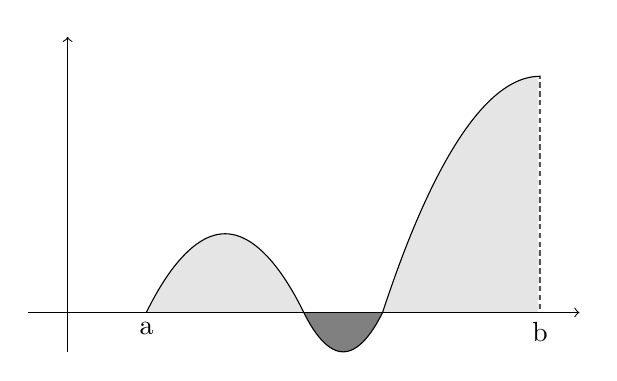
\begin{tikzpicture}


% labels
\draw	(1,0) node[anchor=north] {a}
		(6,0) node[anchor=north] {b};

% vertical axis
\draw[->] (0,-0.5) -- (0,3.5) node[anchor=east] {};


% Psis
\draw [fill=black!10](1,0) parabola bend (2,1) (3,0);
\draw[fill=black!50] (3,0) parabola bend (3.5,-0.5) (4,0);
\draw[fill=black!10] (4,0) parabola bend  (6,3) (6,0);
\draw[dotted,very thick,white] (6,0)--(6,3);
% horizontal axis
\draw[->] (-0.5,0) -- (6.5,0) node[anchor=north] {};
\end{tikzpicture}
\end{center}

Dies ist sehr einfach, wenn die Funktion $f$ überall den konstanten Wert $f(x)=c$ hat für eine feste reelle Zahl $c\in \mathbb{R}$. In diesem Fall ist die Fläche unter dem Graphen von $f$ ein Rechteck und wir definieren dessen Flächeninhalt einfach als Breite mal Höhe, also das Produkt $A=(b-a)c$. Man beachte, dass die Zahl $c$ auch negativ sein darf und dann ist auch A negativ.\\

Eine einfache Formel ergibt sich auch für eine Funktion, die sich aus konstanten Funktionen auf endlich vielen Teilintervalle von $\lbrack a,b\rbrack$ zusammensetzen lässt.

\begin{center}
\begin{tikzpicture}
% horizontal axis
\draw[->] (-0.5,0) -- (6.5,0) node[anchor=north] {};
% labels
\draw	(1,0) node[anchor=north] {a}
		(2.5,0) node[anchor=north] {$a_1$}
		(4,0) node[anchor=north] {$a_2$}
		(5.5,0) node[anchor=north] {b};

% vertical axis
\draw[->] (0,-0.5) -- (0,3.5) node[anchor=east] {};
\draw	(0,3) node[anchor=east] {$c_3$}
		(0,2) node[anchor=east] {$c_2$}
		(0,1) node[anchor=east] {$c_1$};
% 3 columns
\draw (1,0)--(1,1)--(2.5,1);
\draw (2.5,0)--(2.5,3)--(4,3);
\draw (4,0)--(4,3);
\draw (4,2)--(5.5,2);
\draw (5.5,0)--(5.5,2);
%dotted lines
\draw[dotted, very thick] (0,1)--(1,1);
\draw[dotted, very thick] (0,2)--(4,2);
\draw[dotted, very thick] (0,3)--(2.5,3);

\end{tikzpicture}
\end{center}

Für allgemeine beschränkte Funktionen kann man nun wie in II) vorgehen.

\begin{center}
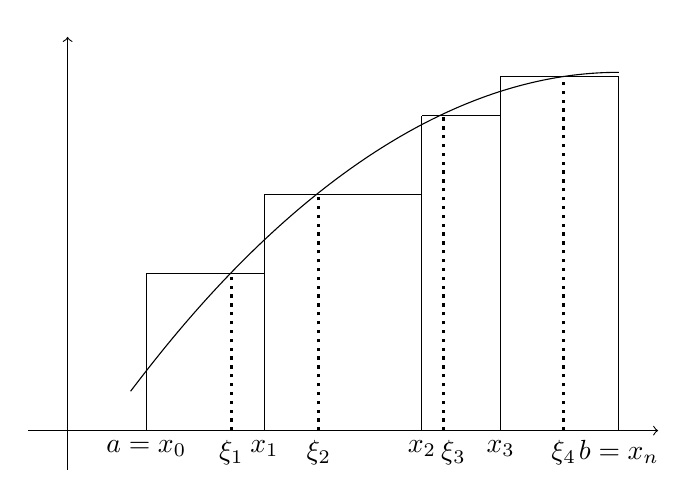
\begin{tikzpicture}
% horizontal axis
\draw[->] (-0.5,0) -- (7.5,0) node[anchor=north] {};
% labels
\draw	(1,0) node[anchor=north] {$a=x_0$}
		(2.5,0) node[anchor=north] {$x_1$}
		(4.5,0) node[anchor=north] {$x_2$}
		(5.5,0) node[anchor=north] {$x_3$}
		(7,0) node[anchor=north] {$b=x_n$};

% vertical axis
\draw[->] (0,-0.5) -- (0,5) node[anchor=east] {};
% 3 columns
\draw (1,0)--(1,2)--(2.5,2);
\draw (2.5,0)--(2.5,3)--(4.5,3);
\draw (4.5,0)--(4.5,4);
\draw (4.5,4)--(5.5,4);
\draw (5.5,0)--(5.5,4.5)--(7,4.5)--(7,0);

\draw (0.8,0.5) parabola bend (7,4.55)(7,4.55);

\draw [dotted, very thick] 
(2.08,0)--(2.08,2)
(3.19,0)--(3.19,3)
(4.77,0)--(4.77,4)
(6.3,0)--(6.3,4.5)
;

\draw	(2.08,0) node[anchor=north] {$\xi_1$}
		(3.19,0) node[anchor=north] {$\xi_2$}
		(4.9,0) node[anchor=north] {$\xi_3$}
		(6.3,0) node[anchor=north] {$\xi_4$};

\end{tikzpicture}
\end{center}

Wir wählen eine Aufteilung (Zerlegung, Einteilung, Partition) des Intervals $I=\lbrack a,b\rbrack$ in endlich viele Teilintervale. \\

Aus jedem dieser Teilintervalle $I_k$ ersetzen wir $f$ durch eine Funktion die auf diesem Teilinterval konstant ist und in einem noch zu klärenden Sinn nicht allzu stark von $f$ abweicht. Dann bilden wir die Summe der Flächeninhalte der auf diese Weise erhaltenen Rechtecke. Diese Summe ist als Näherungswert für die gewünschte Fläche zu verstehen. \\

Um den genauen Wert der Fläche festzulegen bilden wir immer feinere Zerlegungen des Intervalls. Es ist dann das Grenzwertverhalten der diesen Summen zu untersuchen. 
\end{enumerate}
\section{Riemann Integral: Definition, elementare Eigenschaften}
\begin{enumerate}
\item Sei $f: \lbrack a,b\rbrack\rightarrow\mathbb{R}$ eine beschränkte Funktion.\\

\begin{definition}{6.1}
Eine Partition (oder Zerlegung, Einteilung, Unterteilung) eines Intervalls $\lbrack a,b\rbrack$ ist eine endliche Menge $P=\{a=x_0,x_1.\dots,x_n=b \}\\
x_0 < x_1 < x_2 < \dots < x_n$ \\
$P(I):=\{P\subset I \mid a,b\in P, P \text{ ist endlich}\}$ die Menge alle Partitionen \begin{center}
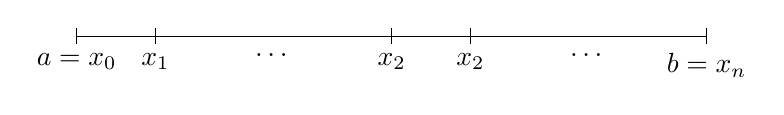
\begin{tikzpicture}
%axis
\draw[] (0,0) -- (8,0) node[anchor=north] {};
% labels
\draw	(0,-0.1) node[anchor=north] {$a=x_0$}
		(8,-0.1) node[anchor=north] {$b=x_n$}	
		(1,-0.1) node[anchor=north] {$x_1$}
		(4,-0.1) node[anchor=north] {$x_2$}
		(5,-0.1) node[anchor=north] {$x_2$}
		(2.5,-0.1) node[anchor=north] {\dots}
		(6.5,-0.1) node[anchor=north] {\dots}		
		;
\draw
	(0,-0.1)--(0,0.1)
	(8,-0.1)--(8,0.1)
	(1,-0.1)--(1,0.1)
	(4,-0.1)--(4,0.1)
	(5,-0.1)--(5,0.1)
	;
\end{tikzpicture}
\end{center}
\end{definition}

Die Feinheit der Zerlegung $P$ ist dabei definiert durch $$\delta (P):=max(x_i - x_{i-1}), 1\leq i \leq n$$ d.h. $\delta (P)$ ist die Länge des grössten Teilintervalls $I_i:=\lbrack x_i,x_{i-1}\rbrack , k=i,\dots,n$

\item Wahl $\xi_i$ von Zwischenpunkten  $x_{i-1} \leq \xi_i  \leq x_i, 1\leq i \leq n$.\\
Jede Summe der Form $$S(f,P,\xi):=\sum\limits_{T = i}^n {f({\xi _i})} ({x_i} - {x_{i - 1}})$$ nennt man eine \textbf{Riemannsche Summe} der Zerlegung P und $\xi$.\\
Die Summe $$U(f,P):=\sum\limits_{i = 1}^n {(\mathop {{\text{Inf }}f}\limits_{[{x_i},{x_{i - 1}}]} )} ({x_i} - {x_{i - 1}})$$ nennt man die \textbf{Untersumme} von $f(x)$ zur Zerlegung $P$, und $$O(f,P):=\sum\limits_{i = 1}^n {f(\mathop {{\text{Sup}}f}\limits_{[{x_{i - 1}},{x_{i}}]} )} ({x_i} - {x_{i - 1}})$$ nennt man die \textbf{Obersumme} von $f(x)$ zur Zerlegung $P$.

\begin{center}
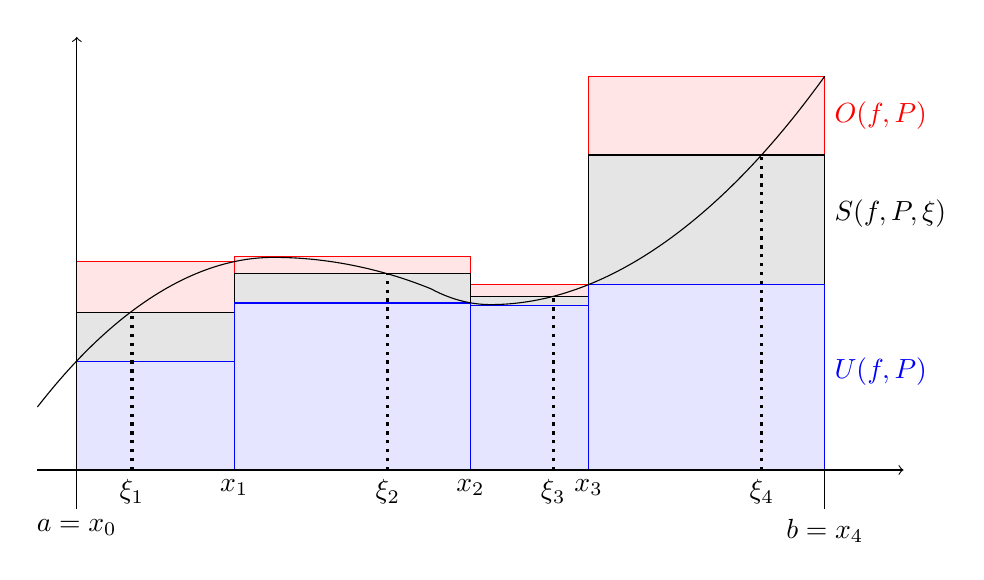
\begin{tikzpicture}
\filldraw[draw=red, fill=red!10] (0,0) rectangle ++(2,2.65);
\filldraw[draw=red, fill=red!10] (2,0) rectangle ++(3,2.71);
\filldraw[draw=red, fill=red!10] (5,0) rectangle ++(1.5,2.35);
\filldraw[draw=red, fill=red!10] (6.5,0) rectangle ++(3,5);

\filldraw[draw=black, fill=black!10] (0,0) rectangle ++(2,2);
\filldraw[draw=black, fill=black!10] (2,0) rectangle ++(3,2.5);
\filldraw[draw=black, fill=black!10] (5,0) rectangle ++(1.5,2.2);
\filldraw[draw=black, fill=black!10] (6.5,0) rectangle ++(3,4);


\filldraw[draw=blue, fill=blue!10] (0,0) rectangle ++(2,1.38);
\filldraw[draw=blue, fill=blue!10] (2,0) rectangle ++(3,2.12);
\filldraw[draw=blue, fill=blue!10] (5,0) rectangle ++(1.5,2.09);
\filldraw[draw=blue, fill=blue!10] (6.5,0) rectangle ++(3,2.35);

% horizontal axis
\draw[->] (-0.5,0) -- (10.5,0) node[anchor=north] {};
% labels
\draw	(0,-0.5) node[anchor=north] {$a=x_0$}
		(9.5,-0.5) node[anchor=north] {$b=x_4$}
		
		(2,0) node[anchor=north] {$x_1$}
		(5,0) node[anchor=north] {$x_2$}
		(6.5,0) node[anchor=north] {$x_3$}
		
		(0.7,0) node[anchor=north] {$\xi_1$}
		(3.95,0) node[anchor=north] {$\xi_2$}
		(6.05,0) node[anchor=north] {$\xi_3$}
		(8.7,0) node[anchor=north] {$\xi_4$}
		
		
		;

% vertical axis
\draw[->] (0,-0.5) -- (0,5.5) node[anchor=east] {};
\draw [](-0.5,0.8) parabola bend (2.5,2.7)(4.5,2.3);
\draw [](4.5,2.3) parabola bend (5.25,2.1)(9.5,5); 

\draw[dotted, very thick] (0.7,0)--(0.7,2);
\draw[dotted, very thick] (3.95,0)--(3.95,2.5);
\draw[dotted, very thick] (6.05,0)--(6.05,2.2);
\draw[dotted, very thick] (8.7,0)--(8.7,4);

\draw	(9.5,4.5) node[anchor=west] {$\color{red}O(f,P)$}
		(9.5,3.25) node[anchor=west] {$\color{black}S(f,P,\xi)$}
		(9.5,1.25) node[anchor=west] {$\color{blue}U(f,P)$};
		
\draw (9.5,0)--(9.5,-0.5);

\end{tikzpicture}
\end{center}

\end{enumerate}

\subsubsection*{Bemerkung 6.2}
Aus den Definitionen folgt direkt
\begin{enumerate}[\indent a)]
\item Für eine feste Zerlegung $P$ gilt stets $U(f,P) \leq S(f,P,\xi) \leq O(f,P)$
\item Für zwei Partitionen $P,Q \in P(I)$ gilt die Ungleichung $P\subset Q \Rightarrow U(f,P) \leq U(f,Q) \leq O(f,Q)\leq O(f,P)$.
\end{enumerate}

\subsubsection*{Beweis} 
Um dies zu verstehen, ist es nützlich, den Fall zu betrachten, dass die Zerlegung $Q$ genau einen Punkt mehr enthält als $P$.\\

Sei $P=\{x_0,\dots ,x_N\}$ und $Q=P\cup \{\xi\}$, wobei $\xi$ ein neuer Unterteilungspunkt, also nicht gleich einem der Elemente von $P$ ist. Dann gibt es genau ein $l\in \{ 1,\dots,N\}$ so dass $x_{l-1}<\xi <x_l$ ist. Damit erhält man $$(\mathop {\sup {\text{ }}f}\limits_{[{x_{l - 1}},\xi ]} )(\xi  - {x_{l - 1}}) + (\mathop {\sup {\text{ }}f}\limits_{[\xi ,{x_l}]} )({x_l} - \xi ) \le (\mathop {\sup {\text{ }}f}\limits_{[{x_{l - 1}},{x_l}]} )({x_l} - {x_{l - 1}})$$


\begin{center}
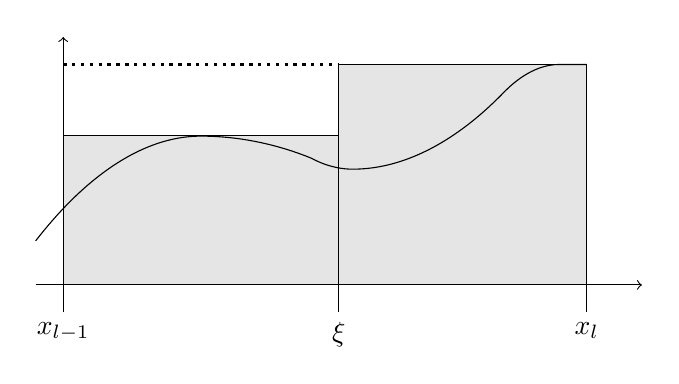
\begin{tikzpicture}[scale=0.7]
\filldraw[draw=black, fill=black!10] (0,0) rectangle ++(5,2.71);
\filldraw[draw=black, fill=black!10] (5,0) rectangle ++(4.5,4);
% horizontal axis
\draw[->] (-0.5,0) -- (10.5,0) node[anchor=north] {};
% labels
\draw	(0,-0.5) node[anchor=north] {$x_{l-1}$}
		(9.5,-0.5) node[anchor=north] {$x_l$}
		(5,-0.5) node[anchor=north] {$\xi$}
		
		;

% vertical axis
\draw[->] (0,-0.5) -- (0,4.5) node[anchor=east] {};
\draw [](-0.5,0.8) parabola bend (2.5,2.7)(4.5,2.3);
\draw [](4.5,2.3) parabola bend (5.25,2.1)(8,3.5); 
\draw [](8,3.5) parabola bend (9,4)(9.5,4);


\draw (9.5,0)--(9.5,-0.5);
\draw (5,0)--(5,-0.5);
\draw[dotted, very thick] (0,4)--(5,4);

\end{tikzpicture}
\end{center}


Addiert man dazu alle Summanden in $$O(f,P)=\sum\limits_i {(\mathop {\sup {\text{ }}f}\limits_{[{x_{i - 1}},{x_i}]} )({x_i} - {x_{i - 1}})} $$
mit $t\neq l$ so ergibt sich die Ungleichung $$O(f,Q)\leq O(f,P)$$
Ebenso beweist man $U(f,Q)\geq U(f,P)$. Damit ist b) für den Fall bewiesen, dass $Q$ genau ein Element mehr als $P$ enthält. Der allgemeine Fall lässt sich hierauf leicht durch vollständige Induktion zurückführen. 

\subsubsection*{Lemma 6.3} Sei $f:I:=\lbrack a,b \rbrack \rightarrow \mathbb{R}$ eine beschränkte Funktion. Dann gilt $$\mathop {\sup {\text{ }}U}\limits_{P \in P(I)} (f,P) \le \mathop {\inf {\text{ }}O}\limits_{P \in P(I)} (f,P)$$

\subsubsection*{Beweis}
Aus $$P\subset Q \Rightarrow U(f,P) \leq U(f,Q) \leq O(f,Q) \leq O(f,P)$$ folgt, dass die Zahl $O(f,Q)$ für jede Partition $Q\in P(I)$ eine obere Schranke für die Menge $\{ U(f,P)\mid P\in P(I)\}$ ist. Also folgt aus der Definition des Supremums als kleinste obere Schranke, dass $\mathop {\sup {\text{ }}U}\limits_{P \in P(I)} (f,P) \le \mathop O(f,Q)$ ist. \\
\newpage
Diese Ungleichung gilt für jede Partition $Q\in P(I)$. Das heisst wiederum, dass die Zahl $\mathop {\sup {\text{ }}U}\limits_{P \in P(I)} (f,P)$ eine untere Schranke für die Menge $\{ O(f,Q)\mid Q \in P(I)\} $ ist.\\

Also folgt aus der Definition der Infimums als grösste untere Schranke, dass die Gleichung $\mathop {\sup U}\limits_{P \in P(I)} (f,P) \le \mathop {\inf O}\limits_{Q \in P(I)} (f,Q)$ ist. Damit ist Lemma 6.3 bewiesen.
\begin{definition}{6.4}
\begin{enumerate}[\indent 1)]
\item Für beschränktes $f=\lbrack a,b \rbrack\rightarrow \mathbb{R}$ bezeichnen 
$$\int\limits_{\underline{a}}^b {fdx = \sup \{ U(f,P):P \in P(I)\} }$$
$$\int\limits_{a}^{\overline{b}} {fdx = \inf \{ O(f,P):P \in P(I)\} }$$
das Untere und Obere Integral von $f$.
\item Ein solches $f$ heisst über $\lbrack a,b\rbrack$ \underline{Riemann - Integrabel} falls $$\int\limits_{\underline{a}}^b {fdx}  = \int\limits_a^{\overline{b}} {fdx} $$ In diesem Fall heisst $A = \int\limits_a^b {fdx} $ das \underline{Riemann Integral von $f$} über den Interval $\lbrack a,b\rbrack$
\end{enumerate}
\end{definition}

\subsubsection*{Beispiel 6.5}
\begin{enumerate}[\indent 1)]
\item Sei $c\in \mathbb{R}$, $f:I\rightarrow \mathbb{R}$ die konstante Funktion mit dem Wert $c$, das heisst $f(x)=c, \forall x\in I$. Dann gilt $$U(f,P)=O(f,P)=(b-a)c, \forall P\in P(I)$$ $\Rightarrow$ $f$ ist Riemann integrierbar und $$\int\limits_a^b {fdx}  = \int\limits_a^b {cdx = c(b - a)} $$ In diesem einfachen Fall stimmt unsere Definition mit der Interpretation des Flächeninhalts als Breite mal Höhe überein. Man beachte, dass die Konstante $c$ auch negativ sein darf. 
\item $f(x) = \left\{ {\begin{array}{*{20}{c}}
{0{\text{ für }}x \ne {x_0}}\\
{1{\text{ für }}x = {x_0}}
\end{array}} \right.{x_0} \in [a,b]$

\begin{center}
\begin{tikzpicture}[scale=0.5]

%axis
\draw[->] (0,-0.5) -- (0,4.5) node[anchor=east] {};
\draw[->] (-0.5,0) -- (9,0) node[anchor=north] {};
% labels
\draw	(1,-0.2) node[anchor=north] {$a$}
		(8,-0.2) node[anchor=north] {$b$}		
		;


\draw[dotted, very thick] (0,4)--(4.5,4);
\draw[dotted, very thick] (4.5,0)--(4.5,4);
\draw[very thick] (1,0)--(8,0);

\filldraw[color=black] (4.5,0) circle (0.1);
\filldraw[color=white] (4.5,0) circle (0.05);
\filldraw[color=black] (4.5,4) circle (0.1);

\end{tikzpicture}
\end{center}



Dann ist f integrierbar mit $$\int\limits_a^b {f(x)dx = 0}$$ denn es gilt $U(f,P)=0$ und $0<O(f,P) \leq 2\delta(P), \forall P$.\\

$O(f,P)$ kann, durch geeignete Wahl der Partition beliebig klein gewählt werden. z.B. $P_n=\{a,a+\frac{{(b - a)}}{n},\dots,b\} \Rightarrow \delta (P)=\frac{b-a}{n}, \mathop {\inf O}\limits_{P \in P(I)}(f,P) = 0$

\item $f(x): = \left\{ {\begin{array}{*{20}{c}}
{1{\text{ für }}x \in [a,b]\backslash \;Q}\\
{0{\text{ für }}x \in [a,b] \cap \;Q}
\end{array}} \right.$
\\

Dann gilt $U(f,P)=0$ und $O(f,P)=1, \forall P\in P(I)$\\
$\Rightarrow f$ ist nicht integrierbar. (f ist beschränkt aber nicht integrierbar)
\end{enumerate}

\subsubsection*{Satz 6.6 (Riemannsches Kriterium für Integrierbarkeit)}
Sei $f:I\rightarrow\mathbb{R}$ eine beschränkte Funktion. Dann sind folgende Aussagen äquivalent
\begin{enumerate}
\item $f(x)$ ist integrierbar über $\lbrack a,b\rbrack$
\item Für jedes $\varepsilon>0$ existiert eine Partition $Q\in P(I)$ mit $$O(f,Q)-U(f,Q)<\varepsilon$$
\end{enumerate}
\subsubsection*{Beweis}
((a)$\Rightarrow$(b))\\
Sei $f$ Riemann integrierbar, $A: = \int\limits_a^b {f(x)dx = \sup U(f,P) = \inf O(f,P)}$\\
Nach definition von sup und inf folgt dass zwei Partitionen $P_1,P_2\in P(I)$ existieren, so dass 

\begin{enumerate}[\indent $(i)$]
\item $A-\frac{\varepsilon}{2}<U(f,P_1)$
\item $O(f,P_2)<A+\frac{\varepsilon}{2}$
\item $U(f,P_1) \leq U(f,Q) < O(f,Q) \leq O(f,P_2)$ 
\end{enumerate} 




Definiere $Q:=P_1\cup P_2$. Dann $P_1\subset Q$ und $P_2 \subset Q$.\\
Nach Bemerkung 6.2b) folgt

$$(i),(ii),(iii) \Rightarrow A-\frac{\varepsilon}{2}<U(f,Q)\leq O(f,Q)<A+\frac{\varepsilon}{2}$$
$$\Rightarrow O(f,Q)-U(f,Q) < \varepsilon$$\\

\noindent((b)$\Rightarrow$(a))\\
Für alle $P\in P(I)$ \[0 \le \underbrace {\int\limits_{\underline{a}}^b {f(x)dx} }_{\inf O(f,P)} - \underbrace {\int\limits_a^{\overline{b}} {f(x)dx} }_{\sup U(f,P)} \le O(f,P) - U(f,P)\]
Aus (b) folgt das $\forall\varepsilon>0$ $$0 < \int\limits_a^{\overline{b}} {f(x)dx - \int\limits_{\underline{a}}^b {f(x)dx < \varepsilon } } \Rightarrow \int\limits_a^{\overline{b}} {f(x)dx = \int\limits_{\underline{a}}^b {f(x)dx} } $$ $\Rightarrow f$ ist integrierbar.

\subsubsection*{Satz 6.7}
\begin{enumerate}
\item Jede Stetige Funktion $f:I\rightarrow \mathbb{R}$ ist R. Integrierbar.
\item Jede Monotone Funktion ist R. Integrierbar.
\end{enumerate}
\subsubsection*{Beweis}
\begin{enumerate}
\item $f:I\rightarrow\mathbb{R}$ stetig, $I=\lbrack a,b\rbrack$ kompakt, $\Rightarrow f$ gleichmässig stetig.\\
d.h. zu jedem $\varepsilon >0$. gibt es $\delta >0$ mit $$\left| {x - y} \right| < \delta  \Rightarrow \left| {f(x) - f(y)} \right| < \frac{\varepsilon }{{b - a}}$$
Für eine $P\in P(I)$ mit Feinheit $\delta(P)<\delta$ gilt dann $$O(f,P)-U(f,P)=\sum\limits_{i = 1}^n {(\mathop {\sup f}\limits_{[{x_{i - 1}},{x_i}]}  - \mathop {\inf f}\limits_{[{x_{i - 1}},{x_i}]} )} ({x_{i - 1}} - {x_i}) $$$$\le \sum\limits_{i = 1}^n {\frac{\varepsilon }{{b - a}}({x_i} - {x_{i - 1}}) = \frac{\varepsilon }{{b - a}}\sum\limits_{i = 1}^n {({x_i} - {x_{i - 1}})} }  = \varepsilon $$
Somit ist $f$ nach Riemannsche Kriterium integrierbar.

\item Sei $f$ monoton wachsend, $P\in P(I)$ eine uniforme Partition mit $$x_i = a+\left(\frac{b-a}{n}\right)i, 0\leq i \leq n$$
$$O(f,P) - U(f,P) = \sum\limits_{i = 0}^{n - 1} {(f({x_{i + 1}}) - f({x_i}))({x_{i + 1}} - {x_i})} $$$$ = \frac{{b - a}}{n}\sum\limits_{i = 0}^{n - 1} {(f({x_{i + 1}}) - f({x_i}))} $$ $$ = \frac{{b - a}}{n}(f(b) - f(a)) < \varepsilon $$
Für jede $\varepsilon>0$, haben wir $\frac{{(b - a)(f(b) - f(a))}}{n} < \varepsilon$. Nach dem Riemannschem Kriterium ist $f$ Integrierbar. (Monoton fallend ist analog). 
\end{enumerate}

\subsubsection*{Satz 6.8 (Riemannsche Summe)}
Sei $f:I\rightarrow \mathbb{R}$ eine beschränkte Funktion. Folgende Aussagen sind äquivalent.
\begin{enumerate}[\indent I)]
\item $f$ ist Riemann Integrierbar und $A: = \int\limits_a^b {f(x)dx} $
\item Für jedes $\varepsilon>0$, existiert eine Zahl $\xi>0$, so dass für jede Partition $P_i=\{x_0,x_1,\dots,x_N\}$ von $I$ und alle $\xi_i,\dots,\xi_N \in \mathbb{R}$ gilt $$\mathop {\delta (P) < \delta }\limits_{{x_{k - 1}} \le {\xi _k} \le {x_k},\forall k}  \Rightarrow \left| {A - \sum\limits_{k = 1}^N {f({\xi _k})({x_k} - {x_{k - 1}})} } \right| < \varepsilon $$
\end{enumerate}
Dieser Satz lässt sich auch so formulieren: Eine beschränkte Funktion $f:I\rightarrow\mathbb{R}$ ist genau dann Riemann integrierbar wenn der Grenzwert $$\mathop {\mathop {\lim }\limits_{\delta (P) \to 0} }\limits_{{\xi _k} \in [{x_{k - 1}},{x_k}]} \sum\limits_{k = 1}^N {f({\xi _k})({x_k} - {x_{k - 1}})} $$ und dann haben wir $$A=\int\limits_a^b {f(x)dx = \mathop {\lim }\limits_{\delta (P) \to 0} } S(f,P,\delta )$$

\subsubsection*{Beweis} Siehe D.Salomon: Das Riemannsche Integrale (Satz 3.1).
\subsubsection*{Korollar 6.8}
Seien $f:\lbrack a,b\rbrack\rightarrow\mathbb{R}$ eine beschränkte und integrierbare Funktion. $\{ P^{(n)}\}$ eine Folge von Partitionen der Intervals $\lbrack a,b\rbrack$ mit $\delta(P^{(n)})\rightarrow 0$ für $n\rightarrow\infty$ und $\{\xi^{(n)}\}$ eine Feste Wahl von Zwischenpunkten zur Partition $P^{(n)}$. Dann ist
\[\int\limits_a^b {f(x)dx = \mathop {\lim }\limits_{n \to \infty } S(f,{P^{(n)}},{\xi ^{(n)}})} \]
\subsubsection*{Beweis}
Wegen Satz 6.8 existiert zu jedem $\varepsilon>0$, ein $\delta>0$ derart, das für alle Partitionen $\delta(P)<\delta$ die Ungleichung 
\[\left| {S(f,P,\xi ) - \int\limits_a^b {f(x)dx} } \right| < \varepsilon \]
gilt und zwar bei beliebiger Wahl der Zwischenpunkten.\\
Wegen  $\delta(P^{(n)})\rightarrow 0$ existiert ein $N\in\mathbb{N}$ mit $\delta(P^{(n)})<\delta$ für alle $n\geq N$.
Für jedes $n\geq N$ ist daher \[\left| {S(f,{P^{(n)}},\xi ) - \int\limits_a^b {f(x)dx} } \right| < \varepsilon \] voraus sich die Behauptung unmittelbar ergibt. 
\subsubsection*{Beispiel}
\[\int\limits_0^1 {({x^2} - x)dx = ?} \]
$$f(x) = {x^2} - x \text{ stetig }\Rightarrow\text{ $f$ integrierbar}$$
Wir wenden Korollar 6.8 an. Wir betrachten die Folge $\{ P^{(n)}\}$ von äquidistanten Partition des intervals $\lbrack 0,1\rbrack$ mit \[x_k^{(n)}: = \frac{k}{n},\text{\indent}\forall k = 0,1, \ldots ,n\]
Dann $\delta(P^{(n)})=\frac{1}{n}\rightarrow 0$ für $n\rightarrow\infty$. Wir wählen die Zwischenpunkte 
\[\xi _k^{(n)}: = \frac{k}{n},\text{\indent}\forall k = 1, \ldots ,n\]

Die $\xi _k^{(n)}$ sind die rechten Endpunkte der Teilintervale $I_{k-1}:=\lbrack \frac{k-1}{n},\frac{k}{n}\rbrack$. Hiermit folgt

$$S(f,{P^{(n)}},{\xi ^{(n)}}) = \sum\limits_{k = 1}^n {f(\xi _k^{(n)})(x_k^{(n)} - x_{k - 1}^{(n)}} )$$
 $$= \sum\limits_{k = 1}^n {\left( {\frac{{{k^2}}}{{{n^2}}} - \frac{k}{n}} \right)\left( {\frac{k}{n} - \frac{{k - 1}}{n}} \right)} $$
$$ = \frac{1}{n}\sum\limits_{k = 1}^n {\left( {\frac{{{k^2}}}{{{n^2}}} - \frac{k}{n}} \right)} $$
$$ = \frac{1}{{{n^3}}}\sum\limits_{k = 1}^n {{k^2}}  - \frac{1}{{{n^2}}}\sum\limits_{k = 1}^n k $$
$$ = \frac{1}{{{n^3}}}\left( {\frac{{n(n + 1)(2n + 1)}}{6}} \right) - \frac{1}{{{n^2}}}\left( {\frac{{n(n + 1)}}{2}} \right)$$
 $$\to \frac{2}{6} - \frac{1}{2} =  - \frac{1}{6}$$
$$ \Rightarrow \int\limits_0^1 {({x^2} - x)dx =  - \frac{1}{6}} $$

%%%%%%%%%%%%%%%%%%%%
\subsection*{Eigenschaften des Integrals}
\subsubsection*{Satz 6.9}
Seien $a<c<b$ und $\alpha, \beta \in \mathbb{R}$ und $f,g:I=\lbrack a,b \rbrack\rightarrow\mathbb{R}$ zwei Reimann Integrierbare Funktionen. Dann gilt folgendes:
\begin{enumerate}
\item Die Funktion $\alpha f + \beta g$ ist integrierbar mit $$\int\limits_a^b {(\alpha f + \beta g)dx = \alpha \int\limits_a^b {f(x)dx + \beta \int\limits_a^b {g(x)dx} } } $$
\item Wenn $f,g$ die Ungleichung $f(x)\leq g(x), \forall x\in\lbrack a,b\rbrack$ erfüllen, dann gilt \[\int\limits_a^b {f(x)dx \le \int\limits_a^b {g(x)dx} } \]
\item $\left| f \right|$ sind R. Integrierbar und $$\left| {\int\limits_a^b {f(x)dx} } \right| \le \int\limits_a^b {\left| {f(x)} \right|dx} $$
\item Das Produkt $fg$ ist Integrierbar.
\end{enumerate}

\subsubsection*{Bemerkung 6.10}
Wir bezeichnen die Menge aller Riemann integrierbaren Funktionen $f:I\rightarrow \mathbb{R}$ mit $R(I):=\{f:I\rightarrow\mathbb{R}\mid f$ R.Integrierbar $\}$. Nach Satz 6.9 i), ist dies ein reeler Vektorraum. $R(I)$ ist ein Unterraum des Vektorraumes aller reelwertigen Funktion $$F(I):=\{ f:I\rightarrow \mathbb{R}\}$$$$C(I):=\{ f:I\rightarrow\mathbb{R}\mid f \text{ stetig}\}$$
ist ein Unterraum von $R(I)$ $$C(I)\subset R(I)\subset F(I)$$
\subsubsection*{Beweis 6.9}
\begin{enumerate}
\item Setze $h:=\alpha f + \beta g$ und sei $\varepsilon>0$ beliebig gegeben. Da $f$ und $g$ integrierbar sind, existieren wegen Riem. Kriterium (Satz 6.6).\\ Partitionen $P_1$ und $P_2 \in P(I)$ mit \[O(f,{P_1}) - U(f,{P_1}) < \frac{\varepsilon }{{(\left| \alpha  \right| + \left| \beta  \right|)}}\] und  \[O(g,{P_2}) - U(g,{P_2}) < \frac{\varepsilon }{{(\left| \alpha  \right| + \left| \beta  \right|)}}\] Aus der Definition von $h$ folgt zunächst \[\left| {h(x) - h(y)} \right| \le \left| \alpha  \right|\left| {f(x) - f(y)} \right| + \left| \beta  \right|\left| {g(x) - g(y)} \right|\] Mit der verfeinerte Partition $P:=P_1\cup P_2$ ergibt sich unter Verwendung von (\textasteriskcentered), wobei 


\[
\mathop {\sup h(x)}\limits_{x \in I}  - \mathop {\inf h(x)}\limits_{x \in I}  = \sup \{ h(x) - h(y)\mid x,y \in I\}\tag{\textasteriskcentered}
\] 




% \begin{enumerate}[(\textasteriskcentered)]
% \item $\text{\hspace{10mm}}\mathop {\sup h(x)}\limits_{x \in I}  - \mathop {\inf h(x)}\limits_{x \in I}  = \sup \{ h(x) - h(y)\mid x,y \in I\}$ 
% \end{enumerate}

Für beschränkte funktion $h$ auf einen intervall $I$ gilt
\[O(h,P) - U(h,P) = \sum\limits_{k = 1}^n {(\mathop {\sup h}\limits_{[{x_{k - 1}},{x_k}]}  - \mathop {\inf h}\limits_{[{x_{k + 1}},{x_k}]} )({x_k} - {x_{k - 1}})} \]
\[\mathop  = \limits^ *  \sum\limits_{x,y \in {I_k}} {\sup \left| {h(x) - h(y)} \right|({x_k} - {x_{k - 1}})} \]
\[ \le \left| \alpha  \right|\sum {\mathop {\sup }\limits_{x,y \in {I_k}} \left| {f(x) - f(y)} \right|({x_k} - {x_{k - 1}})} + \left| \beta  \right|\sum {\mathop {\sup }\limits_{x,y \in {I_k}} \left| {g(x) - g(y)} \right|({x_k} - {x_{k - 1}})} \]
\[ = \left| \alpha  \right|\sum\limits_{k = 1}^n {(\sup f - \inf f)({x_k} - {x_{k - 1}}) + } \left| \beta  \right|\sum\limits_{k = 1}^n {(\sup g - \inf g)({x_k} - {x_{k - 1}})} \]
\[ = \left| \alpha  \right|[O(f,P) - U(f,P)] + \left| \beta  \right|[O(g,P) - U(g,P)] $$ $$< \left| \alpha  \right|\frac{\varepsilon }{{(\left| \alpha  \right| + \left| \beta  \right|)}} + \left| \beta  \right|\frac{\varepsilon }{{(\left| \alpha  \right| + \left| \beta  \right|)}} = \varepsilon \]
Nach Bmk. 6.2 $P_1\subset P$
$$\Rightarrow U(f,P_1)<U(f,P)$$ und $$O(f,P)<O(f,P_1)$$
Dann $$-U(f,P)<-U(f,P_1)$$ und $$O(f,P)-U(f,P)<O(f,P_1)-U(f,P_1)<\frac{\varepsilon}{(\left| \alpha  \right| + \left| \beta  \right|)}$$

\item Seien $f,g:I\rightarrow\mathbb{R}$ integrierbar mit $f(x)\leq g(x), \forall x \in I$.\\
Die Funktion $h:=g-f$ ist wegen (1.) Integrierbar. Sei nur $P=\{x_0,x_1,\dots,x_n\}$ eine beliebige Partition von $\lbrack a,b\rbrack$ folgt dann $\inf h(x) \ge 0,\forall k = 0,1, \ldots ,n$ und daher \[U(h,P) = \sum\limits_P {(\inf h)({x_k} - {x_{k - 1}}) \ge 0} \]
Was wiederum $\int\limits_{\underline{a}}^b {h(x)dx = \sup U(h,P) \ge 0} $ impliziert. \\
Da $h$ aber integrierbar ist, folgt hieraus \[0 \le \int\limits_{\underline{a}}^b {h(x)dx = \int\limits_a^b {h(x)dx} } \]
\[ = \int\limits_a^b {(g(x) - f(x))dx = \int\limits_a^b {g(x)dx - \int\limits_a^b {f(x)dx} } }\geq 0 \]
Dies liefert die Behauptung
\item Nun gilt $ - \left| {f(x)} \right| \le f(x) \le \left| {f(x)} \right|$, $\forall x\in I$\\
Nach (2) folgt daraus die Ungleichung 
\[ - \int\limits_a^b {\left| {f(x)} \right|dx}  \le \int\limits_a^b {f(x)dx}  \le \int\limits_a^b {\left| {f(x)dx} \right|} \]
Diese Ungleichung ist äquivalent zu
\[\left| {\int\limits_a^b {f(x)dx} } \right| < \int\limits_a^b {\left| {f(x)} \right|dx} \]
\item Als Integrierbare Funktionen sind $f$ und $g$ beschränkt. Also existieren die Konstanten 
\[\alpha : = \mathop {\sup }\limits_{x \in [a,b]} \left| {f(x)} \right|{\text{ und }}\beta : = \mathop {\sup }\limits_{x \in [a,b]} \left| {g(x)} \right|\]
Wegen Riem. Kriterium (Satz 6.6) gibt es Partitionen $P_1,P_2$ mit
$$O(f,P_1)-U(f,P_1)<\frac{\varepsilon}{(\alpha + \beta)}, \text{    } O(g,P_2)-U(g,P_2)<\frac{\varepsilon}{(\alpha + \beta)}$$
Setzen wir $h:=fg$ so gilt
\[\left| {h(x) - h(y)} \right| \le \left| {f(x)} \right|\left| {g(x) - g(y)} \right| + \left| {g(y)} \right|\left| {f(x) - f(y)} \right|\]
\[ \le \alpha \left| {g(x) - g(y)} \right| + \beta \left| {f(x) - f(y)} \right|, \forall x,y\in \lbrack a,b\rbrack\]
Sei $P=P_1\cup P_2$.\\
Wie in dem Beweis von (1.) ergibt sich unter verwendung von \[\mathop {\sup }\limits_{x \in I} h - \mathop {\inf }\limits_{x \in I} h = \sup \left\{ {\left| {h(x) - h(y)} \right|x,y \in I} \right\}\]
dann 
$$O(h,P)-U(h,P)$$
\[ = \sum\limits_{k = 1}^n {(\sup h - \inf h)({x_k} - {x_{k - 1}})} \]
\[ = \sum\limits_{k = 1}^n {\mathop {\sup }\limits_{x,y \in {I_k}} \left| {h(x) - h(y)} \right|({x_k} - {x_{k - 1}})} \]
\[ \le \left| \beta  \right|\sum {\mathop {\mathop {\sup }\limits_{{I_k}} \left| {f(x) - f(y)} \right|({x_k} - {x_{k - 1}}) + }} \left| \alpha  \right|\sum {\mathop {\mathop {\sup }\limits_{{I_k}} \left| {g(x) - g(y)} \right|({x_k} - {x_{k - 1}})} } \]
\[ = \left| \beta  \right|\sum {(\mathop {\sup }\limits_{{I_k}} f - \mathop {\inf }\limits_{{I_k}} f)({x_k} - {x_{k - 1}})}  + \left| \alpha  \right|\sum {(\mathop {\sup }\limits_{{I_k}} g - \mathop {\inf }\limits_{{I_k}} g)({x_k} - {x_{k - 1}})} \]
\[ = \left| \beta  \right|[O(f,P) - U(f,P)] + \left| \alpha  \right|[O(g,P) - U(g,P)] < \varepsilon \]

\end{enumerate}

\subsubsection*{Satz 6.10 (Standardabschätzungen)}
Sei $f$ integrierbar über $\lbrack a,b \rbrack$. Dann gelten die Abschätzungen \[(b - a)\mathop {\inf }\limits_{[a,b]} f \le \int\limits_a^b {f(x)dx \le (b - a)\mathop {\sup }\limits_{[a,b]} f} \] 
\subsubsection*{Beweis} 
Für die Partition $P=\{ a,b\}$ von $\lbrack a,b\rbrack$ folgt sofort \[(b - a)\mathop {\inf }\limits_{[a,b]} f = U(f,P) \le \int\limits_a^b {f(x)dx < O(f,P) = (b - a)\mathop {\sup }\limits_{[a,b]} f} \]

\subsubsection*{Satz 6.11}
Sei $f:\lbrack a,b\rbrack\rightarrow\mathbb{R}$ integrierbar. Dann ist $f$ auch auf jedem Teilinterval $\lbrack c,d\rbrack\subseteq\lbrack a,b\rbrack$ integrierbar. \\

\subsubsection*{Beweis}
$f$ ist auf $\lbrack a,b\rbrack$ integrierbar wegen Satz 6.6.\\
Zu jedem $\varepsilon>0$, existiert eine Partition $P'$ von $\lbrack a,b\rbrack$mit $$O(f,P')-U(f,P')<\varepsilon$$
Wir betrachten dann die Verfeinerung $$P'':=P'\cup\{ c,d\}$$
Wegen Bmk. 6.2 haben wir $$O(f,P'')-U(f,P'')<\varepsilon$$
Sei nun $P:=P''\cap \lbrack c,d\rbrack$ die Restriktion der Partition $P''$ auf $\lbrack c,d\rbrack$. Dann gilt mit $g:=f\vline _{\left[ c,d\right] }$ die Abschätzung
\[O(g,P) - U(g,P) = \sum\limits_P {({M_k}(g) - {m_k}(g))({x_k} - {x_{k - 1}})} \]
\[=\sum\limits_P {({M_k}(f) - {m_k}(f))({x_k} - {x_{k - 1}})} \]
\[ \le \sum\limits_{P''} {(M'{'_k}(f) - m'{'_k}(f))({x_k} - {x_{k - 1}})} \]
$$O(f,P'')-U(f,P'')<\varepsilon$$
wobei
\[{M_k}(f): = \mathop {\sup }\limits_{{I_k} \subset P} f\text{\indent}{m_k}(f): = \mathop {\inf }\limits_{{I_k} \subset P} f\]
und, analog
$$M^{''}_{k}\left( f\right) =\sup _{I_k\in P''}f$$

\subsubsection*{Satz 6.12}
Seien $a\leq b\leq c$. Die funktion $f:\lbrack a,c\rbrack\rightarrow\mathbb{R}$ ist genau dann integrierbar falls beide Einschrankungen ${\left. f \right|_{[a,b]}}$ und ${\left. f \right|_{[b,c]}}$ integrierbar sind. In diesem Fall gilt \[\int\limits_a^c {f(x)dx = \int\limits_a^b {f(x)dx + \int\limits_b^c {f(x)dx} } } \]
\subsubsection*{Konvention 6.13}
\begin{enumerate}[\indent 1)]
\item Sei $f$ integrierbar auf einem interval $I$. Für $a\leq b$ in $I$ definiert man \[\int\limits_b^a {f(x)dx =  - \int\limits_a^b {f(x)dx} } \]
Mit diesem Konvention gelten alle bisherigen Eigenschaften. z.B. \[\forall a,b,c \in I:\int\limits_a^c f  = \int\limits_a^b f  + \int\limits_b^c f \]
\item \[\int\limits_a^a {f(x)dx = 0} \]
\end{enumerate}
\section{Differentiation und Integration}
In diesem Kapitel wird dem Zusammenhang zwischen Differentiation und Integration hergestellt. Zu diesem Zweck beginnen wir mit dem folgenden Satz, Mittelwertsatz der Integralrechnung. \\

\subsubsection*{Satz 6.14 (Mws. der Integralrechnung)}
Sei $f:\lbrack a,b\rbrack\rightarrow\mathbb{R}$ eine stetige Funktion. Dann existiert ein $\xi\in\lbrack a,b\rbrack$ mit \[\int\limits_a^b {f(x)dx = f(\xi )(b - a)} \] 

Geometrisch:

\begin{center}
\pgfmathdeclarefunction{poly}{0}{%
      \pgfmathparse{-x^3+5*(x^2)-3*x-3}%
    }

\begin{tikzpicture}
\filldraw[draw=black!15, fill=black!15] (0.79,0) rectangle ++(5.27,3.035);
\begin{axis}[
  xmin=-2,
  xmax=5,
  ymin=-5,
  ymax=10,
  axis y line=left,
  axis x line=bottom,
  xtick={-1.2,2,4.2},
  xticklabels={$a$,$\xi$,$b$},
  ytick={3},
  yticklabels={$f(\xi)$},
  samples=160
]

\addplot[mark=none,help lines,domain=-2:4.2] {3};

% draw graph for the first function f
\addplot+[black,thick,mark=none,domain=-1.2:4.2,stack plots=y] {poly};
% draw graph of max(g-f, 0) and stack
\addplot+[mark=none,fill=gray!70,draw=black,domain=-1.2:4.2,stack plots=y] {max(3-(poly),0)} \closedcycle;
% draw graph of min(g-f, 0) and stack
\addplot+[mark=none,fill=black!60,draw=black,domain=-1.2:4.2,stack plots=y] {min(3-(poly),0)} \closedcycle;

\draw[help lines] (axis cs:-1.2,-5) -- (axis cs:-1.2,3);
\draw[help lines] (axis cs:2,-5) -- (axis cs:2,3);
\draw[help lines] (axis cs:4.2,-5) -- (axis cs:4.2,3);
\end{axis}

\draw	(0.95,3.6) node[anchor=north] {D}
		(2.3,2.5) node[anchor=north] {A}
		(4.9,3.8) node[anchor=north] {C}
		(5.92,3.1) node[anchor=north] {B}
		;
\end{tikzpicture}
\end{center}



\subsubsection*{Beweis}
Wir setzen 
\[m: = \min \{ f(x)\mid x \in [a,b]\}  = f({x_ - })\]
\[M: = \max \{ f(x)\mid x \in [a,b]\}  = f({x_ + })\]
Wegen Satz 6.10
\[m(b - a) \le \int\limits_a^b {f(x)dx \le M(b - a)} \]
\[f({x_ - }) = m \le \frac{1}{{b - a}}\int\limits_a^b {f(x)dx \le M = f({x_ + })} \]
Also $\frac{1}{{b - a}}\int\limits_a^b {f(x)dx \le M} $ für ein $M\in\lbrack m,M\rbrack$. Da $f$ stetig ist, wegen Zwischenwertsatz gibt es $\xi\in\lbrack a,b\rbrack$ mit $f(\xi ) = \frac{1}{{b - a}}\int\limits_a^b {f(x)dx} $. Nun kommt die erste Hauptsatz der Diff- und Integralrechnung.\\

\subsubsection*{Satz 6.15 (Hauptsatz A)}
Sei $f:\lbrack a,b\rbrack\rightarrow\mathbb{R}$ eine stetige Funktion. Definiere für jeder $x\in\lbrack a,b\rbrack$ \[F(x): = \int\limits_x^b {f(t)dt} \]
Dann ist $F:I\rightarrow\mathbb{R}$ differenzierbar und $F'(x)=f(x)\text{, }\forall x \in\lbrack a,b\rbrack$.\\
\subsubsection*{Beweis}
Für jedes $h\neq 0$ ist \[\frac{{F(x + h) - F(x)}}{h} = \frac{1}{h}\left[ {\int\limits_a^{x + h} {f(t)dt}  - \int\limits_a^x {f(t)dt} } \right] \mathop  = \limits^{6.12}  \frac{1}{h}\int\limits_a^{x + h} {f(t)dt} \]
Nach dem Mws der Integralrechnung existiert zu jedem solchen $h\neq 0$ ein Zwischenpunkt $\xi_h\in\lbrack x,x+h\rbrack$ (bzw. $\xi_h\in\lbrack x + h,x\rbrack$ falls $h<0$) mit \[\int\limits_x^{x + h} {f(t)dt = (h)f({\xi _h})} \]
Nun ist $\xi_h \rightarrow x$ für $h\rightarrow 0$. Da $f$ stetig ist $$f(\xi_h)\rightarrow f(x) \text{ für } h\rightarrow 0$$
Damit erhalten wir \[F'(x) = \mathop {\lim }\limits_{h \to 0} \frac{{F(x + h) - F(x)}}{h} = \mathop {\lim }\limits_{h \to 0} \frac{1}{h}\int\limits_x^{x + h} {f(t)dt = } \mathop {\lim }\limits_{h \to 0} \frac{1}{h}(hf({\xi _h})) = f(x)\]
Folgender Begriff ist dann naheliegend. \\

\begin{definition}{6.16}
 Sei $f:\lbrack a,b\rbrack\rightarrow\mathbb{R}$ eine Funktion. Ein Stammfunktion von $f$ (auf $a,b$) ist ein differenzierbare Funktion $F:\lbrack a,b\rbrack\rightarrow\mathbb{R}$ mit $F'(x)=f(x)$.\\
\end{definition}
\noindent Wegen Satz 6.15, hat jede stetige Funktion mindestens eine Stammfunktion. Mit Ausnahme einer additiven Konstante, die beim Differenzieren ja wegfällt, ist die Stammfunktion auch eindeutig bestimmt. Dies ist der Inhalt des folgendes Satzes.\\

\subsubsection*{Satz 6.17}
Seien $I\subset \mathbb{R}$ ein beliebiges Interval und $F:I\rightarrow\mathbb{R}$ eine Stammfunktion von $f:I\rightarrow\mathbb{R}$. Dann gelten:
\begin{enumerate}[\indent (a)]
\item Die Funktion $F+c$ ist für jede Konstante $c\in\mathbb{R}$ ebenfalls eine Stammfunktion von $f$.
\item Ist $G:I\rightarrow\mathbb{R}$ eine weitere Stammfunktion von $f$, so gibt es eine Konstante $c\in\mathbb{R}$ mit $G=F+c$
\end{enumerate}

\subsubsection*{Beweis}
\begin{enumerate}[\indent (a)]
\item Offenbar ist mit $F$ auch $F+c$ differenzierbar und es gilt $(F+c)'=F'=f$
\item Da $F$ und $G$ Stammfunktionen von $f$ sind, gilt $F'=f, G'=f$. Also $(F-G)'=0$ und $F-G=\text{konstante Funktion}$. 
\end{enumerate}

\begin{definition}{6.18}
 Eine Stammfunktion von $f$ heisst auch unbestimmtes Integral von $f$ und wird bezeichnet mit $\int {f(x)dx} $. Mittels einer Stammfunktion lässt sich das Integral einer gegebenen Abbildung sehr leicht berechnen. Dies ist der Inhalt des Hauptsatz B.\\
\end{definition}
\subsubsection*{Satz 6.19 (Hauptsatz der Diff- und Integralberechnung Version B)}
Sei $f:I\rightarrow\mathbb{R}$ eine stetige Funktion und $F$ eine beliebige Stammfunktion von $f$. Dann gilt \[\int\limits_a^b {f(x)dx = F(b) - F(a): = \left. {F(x)} \right|_a^b}\text{,\indent}\forall a,b\in I \]

\subsubsection*{Beweis}
Für $x\in I$ definieren wor $$F_0(x):=\int\limits_a^x {f(t)dt} $$
Dann ist $F_0:I\rightarrow\mathbb{R}$ wegen Satz 6.15 eine (Spezielle) Stammfunktion von $f$ mit \[{F_0}(0) = 0\text{\indent}{F_0}(b) = \int\limits_c^b {f(t)dt} \]
Für die beliebige Stammfunktion $F$ gilt somit $F-F_0=c$ für eine Konstante $c\in\mathbb{R}$. Deshalb ist \[F(b) - F(a) = {F_0}(b) - {F_0}(a) = {F_0}(b) = \int\limits_a^b {f(t)dt} \] womit alles bewiesen ist. \\

Der Satz 6.19 ist das zentrale Ergebnis und zur Berechnung konkreter Integral. Man Benötigt nur eine Stammfunktion uns hat von dieser lediglich die Differenz der Funktionswerte zwischen den beiden Endpunkten des Intervals $\lbrack a,b\rbrack$ zu bilden. 
Insbesondere spielt es keine Rolle, welche Werte die Stammfunktion im Inneren des Intervals  $\lbrack a,b\rbrack$ annimmt.
\subsection*{Beispiele von Stammfunktionen}

%\end{comment}
%\todo{Remove Comment!!}

\subsubsection*{Beispiel 6.20}
\renewcommand{\arraystretch}{1.6}
\begin{tabularx}{\textwidth}{|Y|Y|Y|}
\hline
    Definitions Bereich & Funktion $f$                          & Stammfunktion $F$                                                      \\\hline\hline
    $(0,\infty)$        & $x^\alpha,\text{ }\alpha\in\mathbb{R}$ & $\frac{{{x^{\alpha  + 1}}}}{{\alpha  + 1}} + c,{\rm{ }}\alpha  \ne  - 1$ \\ [1.5ex]
    ~                   & ~                                     & $\log \left| x \right| + c,{\rm{ }}\alpha  =  - 1$                       \\[1.5ex]\hline
    $\mathbb{R}$        & $x^n, n\in\mathbb{N}$                 & $\frac{{{x^{n + 1}}}}{{n + 1}} + c,{\rm{ }}n \in \mathbb{N}$             \\[1.5ex]\hline
    $\mathbb{R}$        & ${e^x}$                             & ${e^x}+c$                                                                \\ [1.5ex]\hline
    $\mathbb{R}$        & $\sin{x}$                             & $-\cos{x}+c$                                                                \\ [1.5ex]\hline
$\mathbb{R}$        & $\cos{x}$                             & $\sin{x}+c$                                                                \\ [1.5ex]\hline
$(-1,1)$        & $\frac{1}{\sqrt{1-x^2}}$                             & $\arcsin{x}+c$                                                                \\ [1.5ex]\hline
$(-1,1)$        & $\frac{-1}{\sqrt{1-x^2}}$                             & $\arccos{x}+c$                                                                \\ [1.5ex]\hline
$\mathbb{R}$        & $\frac{1}{\sqrt{1+x^2}}$                             & $\arctan{x}+c$                                                                \\ [1.5ex]\hline
$(-\frac{\pi}{2},\frac{\pi}{2})$        & $\tan{x}$                             & $- \ln \left| {\cos x} \right| + c$                                                                \\ [1.5ex]\hline
$(0,\pi)$        & $\cot{x}$                             & $\ln \left| {\sin x} \right| + c$                                                                \\[1.5ex]\hline
%Hello \\
$\mathbb{R}$ & $\sinh x$ & $\cosh x + c$\\[1.5ex]\hline
$\mathbb{R}$ & $\cosh x$ & $\sinh x + c$\\[1.5ex]\hline
$\mathbb{R}$ & $\frac{1}{\sqrt{1+x^2}}$  & $\arcsinh x + c$ \\[1.5ex]\hline
$(1,\infty)$ & $\frac{1}{\sqrt{x^2-1}}$ & $\arccosh x + c$ \\[1.5ex]\hline
$\lbrack -1,1\rbrack$ & $\frac{1}{1-x^2}$ & $\arctanh x + c$ \\[1.5ex]\hline
 \end{tabularx}

\subsubsection*{Beispiel}
$$F(x)=-\ln\left| \cos x \right| = -\frac{1}{2}\ln\left(\cos x\right)^2$$
und die Ableitung ist (nach Kettenregel):
\[F'(x) =  - \frac{1}{2}\frac{1}{{\cos {{(x)}^2}}}(2\cos x)( - \sin x) = \frac{{\sin x}}{{\cos x}} = \tan x\]

\section{Partielle Integration}
Da das Integration die Umkehrung von differenzieren ist, liefert jede Ableitungsregel eine für das Integrieren.\\

Partielle Integration ist eine Umkehrung der Leibnizschen Produktregel und besagt für unbestimmte bzw. das bestimmte Integral:
\[\begin{array}{c}
(uv)' = u'v + uv'\\
 \Rightarrow \int {uv'}  = uv - \int {u'v}  + c
\end{array}\]

\subsubsection*{Satz 6.21 (Partielle Integration)}
Seien $f,g:\lbrack a,b\rbrack\rightarrow\mathbb{R}$ zwei stetig differenzierbare Funktionen. Dann gilt 
\[\int {f(x)g'(x)dx = f(x)g(x) - \int {f'(x)g(x)dx} } \]
und
\[\int\limits_a^b {f(x)g'(x)dx = \left. {f(x)g(x)} \right|_a^b - \int\limits_a^b {f'(x)g(x)dx} } \]
\subsubsection*{Beispiel 6.22}
\begin{enumerate}
\item $\int {\underbrace x_u\underbrace {{e^x}}_{v'}dx = x{e^x} - \int {1{e^x}dx} } =x e^x - e^x$
$\left\{\begin{array}{cc} f(x)=x & g'(x)=e^x \\ f'(x)=1 & g(x)=e^x\end{array}\right.$

\item $\int {\underbrace {{x^n}}_u\underbrace {{e^x}}_{v'}dx = {x^n}{e^x} - \int {n{x^{n - 1}}{e^x}dx} } $\\
Durch Induktion über $n\in\mathbb{Z}^{\geq 0}$ folgert man daraus das Resultat \[\int {{x^n}{e^x}dx = {{( - 1)}^n}n!\sum\limits_{k = 0}^n {\frac{{{{( - x)}^k}}}{{k!}}{e^x} + c} } \]

\item Partielle Integration eignet sich gut dazu, Logarithmische terme zu eliminieren.\\
Manchmal muss man dazu den Integranden erst künstich als Produkt schreiben
\[\int {\log xdx = \int {\underbrace {(\log x)}_u\underbrace {(1)}_{v'}dx} } \]
\[ = (\log x)x - \int {\frac{1}{x}} xdx = x\log x - x + c\]

\item Manchmal führt wiederholte partielle Integration auf den ursprünglichen Ausdruck zurück. Mit Glück kann man dann noch diesem auflösen 
\[\int {{{\sin }^2}xdx = \int {\underbrace {(\sin x)}_u\underbrace {(\sin x)}_{v'}dx} } \]
$$ =  - \sin x\cos x + \int {{{\cos }^2}xdx}$$
$$ =  - \sin x\cos x + \int {(1 - {{\sin }^2}x)dx}$$
$$ =  - \sin x\cos x + x - \int {{{\sin }^2}xdx} $$

\[ \Rightarrow 2\int {{{\sin }^2}xdx = x - \sin x\cos x} \]
\[ \Rightarrow \int {{{\sin }^2}xdx = \frac{1}{2}\left( {x - \sin x\cos x}  \right)} \]
Andere möglichkeit:
$$\cos 2x = 1-2\sin^2x=\cos^2x-\sin^2x=2\cos^2x-1$$
$$\sin^2x=\frac{1}{2}(1-\cos 2x)$$
mit $$\cos 2x=\left(\frac{\sin 2x}{2} \right)'$$
Dann: $$\int{\sin^2 x}=\frac{1}{2}\int{1-\cos 2x dx}$$
$$=\frac{1}{2}\left[ x-\int{\cos 2x dx}\right]$$
$$=\frac{1}{2}\left[ x-\frac{\sin 2x}{2}\right] +c$$
$$\sin 2x =2\sin x\cos x$$
\end{enumerate}

\subsubsection*{Beispiel 6.23}
\[\int\limits_0^{\pi /2} {{{(\sin x)}^{k + 1}}dx = \int\limits_0^{\pi /2} {\underbrace {{{(\sin x)}^k}}_u\underbrace {(\sin x)}_{v'}dx} } \]


$$ = \left. {\underbrace {{{(\sin x)}^k}}_u\underbrace {( - \cos x)}_v} \right|_0^{\pi /2} - \int\limits_0^{\pi /2} {\underbrace {k{{(\sin x)}^{k - 1}}(\cos x)}_{u'}} \underbrace {( - \cos x)}_vdx$$
$$ = 0 + k\int\limits_0^{\pi /2} {{{(\sin x)}^{k - 1}}} \left[ {1 - {{\sin }^2}x} \right]dx$$
$$ = k\int\limits_0^{\pi /2} {{{(\sin x)}^{k - 1}} - k\int\limits_0^{\pi /2} {{{(\sin x)}^{k + 1}}dx} } $$


Also:
\[\int\limits_0^{\pi /2} {{{(\sin x)}^{k + 1}}dx = \frac{k}{{(1 + k)}}\int\limits_0^{\pi /2} {{{(\sin x)}^{k - 1}}dx} } \]
Falls $k+1=2n$:

$$\int\limits_0^{\pi /2} {{{(\sin x)}^{2n}}dx = \frac{{2n - 1}}{{2n}}\int\limits_0^{\pi /2} {{{(\sin x)}^{2(n - 1)}}dx} } $$
$$ = \frac{{2n - 1}}{{2n}}\frac{{2n - 3}}{{2n - 2}} \ldots \frac{1}{2}\int\limits_0^{\pi /2} {1dx} $$
$$ = \frac{{(2n)(2n - 1)(2n - 2) \ldots 1}}{{{{\left[ {(2n)(2n - 2) \ldots 2} \right]}^2}}}\frac{\pi }{2}$$
$$ = \frac{{(2n)!}}{{{{({2^n}n!)}^2}}}\frac{\pi }{2}$$

\noindent Analog:
\[\int\limits_0^{\pi /2} {{{(\sin x)}^{2n + 1}}dx = \frac{{{{({2^n}n!)}^2}}}{{(2n + 1)!}}} \]

\noindent Beachte: der $\pi$-Term kommt im Zweiten Fall nicht vor!\\

\noindent Dies benutzen wir wie folgt um ein ``Formel'' für $\pi$ aufzustellen.\\

\noindent Für $0\leq x \leq\pi/2$:

\[{(\sin x)^k} - {(\sin x)^{k + 1}} = {(\sin x)^k}\left[ {1 - \sin x} \right] \ge 0\]
\[ \Rightarrow {(\sin x)^k} \geq {(\sin x)^{k + 1}}\text{\hspace{10mm}} \left( k\geq 0,0\leq x \leq \pi/2\right)\]
Also:
\[\int\limits_0^{\pi /2} {{{(\sin x)}^{2n + 1}}dx \le \int\limits_0^{\pi /2} {{{(\sin x)}^{2n}}dx \le \int\limits_0^{\pi /2} {{{(\sin x)}^{2n - 1}}dx} } } \]
d.h.
\[\frac{{{{({2^n} n!)}^2}}}{{(2n + 1)!}} \le \frac{{(2n)!}}{{{{({2^n}n!)}^2}}} \cdot \frac{\pi }{2} \le \frac{{{{\left( {{2^{n - 1}}(n - 1)!} \right)}^2}}}{{(2n - 1)!}}\]
Also:
\[\frac{{{{({2^n}n!)}^4}}}{{(2n + 1)!}} \cdot \frac{2}{{(2n)!}} \le \pi  \le \frac{{{{({2^n}n!)}^4}}}{{{{(2n!)}^2}}} \cdot \frac{2}{{2n}}\]
\[\frac{{{{({2^n}!)}^4}}}{{(2n + 1)}} \cdot \frac{2}{{{{((2n)!)}^2}}} \le \pi  \le \frac{{{{({2^n}n!)}^4}}}{{{{(2n!)}^2}}} \cdot \frac{2}{{2n}}\]
\[ \Rightarrow \pi  = \mathop {\lim }\limits_{n \to \infty } \frac{1}{n}\frac{{{{({2^n}n!)}^4}}}{{{{(2n!)}^2}}}\text{\hspace{5mm} Wallische Formel.}\]

\subsubsection*{Beispiel 6.24 (Stirlingsche Formel)}
Für $n\geq 2$ sei $\ln (n!) = \sum\limits_{k = 2}^n {\ln (k)} $. Wir zeigen dass man kann $\ln\left| k\right|$ sehr gut durch $\int\limits_{k - 1/2}^{k + 1/2} {\ln xdx} $ approximieren.\\

\noindent Da $$x\ln x-x$$ Stammfunktion von $\ln(x)$ ist, folgt $$\int\limits_{k - 1/2}^{k + 1/2} {\ln xdx}  = \left. {x\ln x - x} \right|_{k - 1/2}^{k + 1/2}$$ Darin kommen also $\ln\left(k+\frac{1}{2}\right)$ sowie $\ln\left(k-\frac{1}{2}\right)$ vor. Wir benutzen nun Taylor:\\

\noindent Falls $g(x)=\ln(x)$ sei $$g(x)=g(x_0)+g'(x_0)(x-x_0)+\frac{g''(x_0)}{2!}(x-x_0)^2+\frac{g^{(3)}(\xi)}{3!}(x-x_0)^3$$ mit $\xi$ zwischen $x$ und $x_0$.\\

\noindent Auf $\left. {\begin{array}{*{20}{c}}
{x = k + \frac{1}{2}}\\
{{x_0} = k}
\end{array}} \right\}$ aufgewendet ergibt:
\[\ln \left( {k + \frac{1}{2}} \right) = \ln k + \frac{1}{{2k}} - \frac{1}{{8{k^2}}} + {t_k}\]
wobei $${t_k} = \frac{2}{{{\xi ^3}}}\frac{1}{{3!}}{\left( {\frac{1}{2}} \right)^3} = \frac{1}{{24{\xi ^3}}}$$
\[\left| {{t_k}} \right| \le \frac{1}{{24{k^3}}}\text{\hspace{10mm}}\xi  \in \left[ {k,k + \frac{1}{2}} \right]\]

\noindent Analog:
\[\ln \left( {k - \frac{1}{2}} \right) = \ln k - \frac{1}{{2k}} - \frac{1}{{8{k^2}}} + {t'_k}\]

\[\left| {{t'_k}} \right| \le \frac{1}{{24{\left(k-\frac{1}{2}\right)^3}}}\]
Also:

\[\int\limits_{k - 1/2}^{k + 1/2} {x\ln x - xdx = \left( {k + \frac{1}{2}} \right)} \left( {\ln k + \frac{1}{{2k}} - \frac{1}{{8{k^2}}} + {t_k}} \right) - \left( {k + \frac{1}{2}} \right)\]
$$ - \left[ {\left( {k - \frac{1}{2}} \right)\left( {\ln k - \frac{1}{{2k}} - \frac{1}{{8{k^2}}} + t{'_k}} \right) - \left( {k - \frac{1}{2}} \right)} \right]$$
$$ = \ln k - \frac{1}{{8{k^2}}} + \left( {k + \frac{1}{2}} \right){t_k} - \left( {k - \frac{1}{2}} \right)t{'_k}$$
$$ = \ln k + {r_k}\text{\hspace{10mm}}\left| {{r_k}} \right| \le \frac{c}{{{k^2}}}$$
\noindent Nun folgt:

\[\ln n! = \sum\limits_{k = 2}^n {\ln k\mathop  = \limits^{( * )} \sum\limits_{k = 2}^n {\int\limits_{k - \frac{1}{2}}^{k + \frac{1}{2}} {\ln xdx} }  - \sum\limits_{k = 2}^n {{r_k}} } \text{\hspace{4mm} mit }( * )=\left( {\int\limits_{k - \frac{1}{2}}^{k + \frac{1}{2}} {\ln xdx = \ln k + {r_k}} } \right) \]
\[ = \underbrace {\int\limits_1^{n + \frac{1}{2}} {\ln xdx} }_{( * )} - \int\limits_1^{\frac{3}{2}} {\ln xdx - \sum\limits_{k = 2}^n {{r_k}} } \]
\[( * ) = \int\limits_1^{n + \frac{1}{2}} {\ln xdx = \left. {x\ln x - x} \right|_1^{n + \frac{1}{2}}}  = \left( {n + \frac{1}{2}} \right)\ln \left( {n + \frac{1}{2}} \right) - \left( {n + \frac{1}{2}} \right) + 1\]
\[ = \left( {n + \frac{1}{2}} \right)\ln \left( {n + \frac{1}{2}} \right) - n + \frac{1}{2}\]
Ersetzen wir $\ln \left( {n + \frac{1}{2}} \right) = \ln n + \frac{1}{{2n}} - \frac{1}{{8{n^2}}} + {t_n}$ so folgt:

\[(*) = \left( {n + \frac{1}{2}} \right)\ln n - n + \left( {n + \frac{1}{2}} \right)\left\{ {\frac{1}{{2n}} - \frac{1}{{8{n^2}}} + {t_n}} \right\} + \frac{1}{2}\]
\[ = \left( {n + \frac{1}{2}} \right)\ln n - n + \frac{1}{2} - \frac{1}{{8{n^2}}} + n{t_n} + \frac{1}{{4n}} - \frac{1}{{16{n^2}}} + \frac{1}{2}{t_n} + \frac{1}{2}\]
\[ = \left( {n + \frac{1}{2}} \right)\ln n - n + 1 + \frac{1}{{8n}} + n{t_n} - \frac{1}{{16{n^2}}} + \frac{1}{2}{t_n}\]

\noindent Also:
\[\ln (n!) = n\ln n + \frac{1}{2}\ln n - n + {a_n}\]
wobei
\[{a_n} = {\frac{1}{{4n}} + \left( {n + \frac{1}{2}} \right)\left( { - \frac{1}{{8{n^2}}} + {t_n}} \right)} + \sum\limits_{k = 2}^n {{r_k} - \int\limits_1^{\frac{3}{2}} {\ln xdx} } \]
und $\left| {{r_k}} \right| \le \frac{c}{{{k^2}}} \Rightarrow \sum\limits_{k = 2}^n {{r_k}} $ konvergiert.\\

\noindent Sei $a:=\lim a_n$, $b=e^a$ und $b_n=e^{a_n}$. Also:
\[\log n! = \left( {n + \frac{1}{2}} \right)\log n - n + {a_n} = \log {n^{n + \frac{1}{2}}} - n + {a_n}\]
folgt 
\[n! = {n^{n + \frac{1}{2}}}{e^{ - n}}{e^{{a_n}}} = \sqrt n {n^n}{e^{ - n}}{e^{{a_n}}} \Rightarrow {b_n} = \frac{{n!}}{{\sqrt n {n^n}{e^{ - n}}}}\]

\noindent Wir möchten jetzt $b:=e^a$ bestimmen:

\[b = \lim {b_n} = \mathop {\lim }\limits_{n \to \infty } \frac{{{b_n}^2}}{{{b_{2n}}}} = \lim {\left( {\frac{{n!}}{{\sqrt n {n^n}{e^{ - n}}}}} \right)^2}\left( {\frac{{\sqrt {2n} {{(2n)}^{2n}}{e^{2n}}}}{{(2n)!}}} \right)\]
\[ = \mathop {\lim }\limits_{n \to \infty } \frac{{{{(n!)}^2}}}{{(2n)!}}\sqrt {\frac{2}{n}} \frac{{{{(2n)}^{2n}}}}{{{n^{2n}}}} = \mathop {\lim }\limits_{n \to \infty } \frac{{{{(n!)}^2}}}{{(2n)!}}\sqrt {\frac{2}{n}} {2^{2n}} = \mathop {\lim }\limits_{n \to \infty } \frac{{{{({2^n}n!)}^n}}}{{(2n)!}} \cdot \frac{{\sqrt 2 }}{{\sqrt n }}\]
\[ = \sqrt {2\pi} \]

Also $b=\sqrt{2\pi}$ womit 
\begin{framed}
\[n! \approx \sqrt {2\pi n} {n^n}{e^{ - n}}\text{\hspace{10mm} Stirling's formel}\]
\end{framed}
\subsubsection*{Beispiel: Der Satz von Taylor}
Die Taylor - Entwicklung eine Funktion $f\in C^{n+1}$ um $x_0$ erhält man durch $n-$fache partielle Integration:
\[f(x) - f({x_0}) = \int\limits_{{x_0}}^x {f'(t)dt = } \int\limits_{{x_0}}^x {\underbrace {{{(x - t)}^0}}_{v'}\underbrace {f'(t)}_udt} \]
\[ = (x - {x_0})f'({x_0}) + \int\limits_{{x_0}}^x {\underbrace {(x - t)'}_{v'}} \underbrace {f''(t)}_udt\]
\[ = (x - {x_0})f'({x_0}) + \frac{{{{(x - {x_0})}^2}}}{2}f''({x_0}) + \frac{1}{2}\int\limits_{{x_0}}^x {{{(x - t)}^2}f'''(t)dt} \]
$$\text{\vdots}$$
\[ = \sum\limits_{k = 1}^n {{{(x - {x_0})}^k}\frac{{{f^{(k)}}({x_0})}}{{k!}}}  + \frac{1}{{n!}}\int\limits_{{x_0}}^x {{{(x - t)}^n}{f^{(n + 1)}}(t)dt} \]
Aus Mittelwertsatz der Integralrechnung bekommt man die Lagrange Restgliedformel.
\[\frac{1}{{n!}}\int\limits_{{x_0}}^x {{{(x - t)}^n}{f^{(n + 1)}}(t)dt}  = \frac{1}{{(n + 1)!}}{f^{n + 1}}(\xi ){(x - {x_0})^{n + 1}}\text{ für ein }\xi\in\lbrack x_0,x\rbrack\]
\newpage
\section{Methode der Substitution}
Methode der Substitution ist eine Umkehrung der Kettenregel.
\subsubsection*{Satz 6.25 (Substitutionsregel)}
Sei 
\begin{itemize}
\item $f:\lbrack a,b\rbrack\rightarrow\mathbb{R}$ stetig
\item $g:\lbrack\alpha,\beta\rbrack\rightarrow\mathbb{R}$ der klasse $C'$
\end{itemize}
Sowie $t_0\leq t_1$ in $\lbrack\alpha,\beta\rbrack$ so dass $g\left(\lbrack t_0, t_1\rbrack\right)\subset\lbrack a,b\rbrack$.
Dann gilt 
\[\int\limits_{g({t_0})}^{g({t_1})} {f(x)dx = \int\limits_{{t_0}}^{{t_1}} {f\left( {g\left( t \right)} \right)g'\left( t \right)dt} } \]

\subsubsection*{Beweis}
Sei $F:\lbrack a,b\rbrack\rightarrow\mathbb{R}$ eine Stammfunktion für $f$. Dann gilt (nach Hauptsatz B)
\[\int\limits_{g({t_0})}^{g({t_1})} {f(x)dx = F\left( {g({t_1})} \right)}  - F\left( {g({t_0})} \right)\]
Nach der Kettenregel, haben wir
\[(F \circ g)'(t) = F'(g(t))g'(t) = f(g(t))g'(t)\]
d.h. $F\circ g$ ist eine Stammfunktion für $f(g(t))g'(t)$. Woraus mit dem Hauptsatz B folgt 
\[\int\limits_{{t_0}}^{{t_1}} {f\left( {g(t)} \right)} g'(t)dt = \left( {F \circ g} \right)({t_1}) - \left( {F \circ g} \right)({t_0}) = F\left( {g({t_1})} \right) - F\left( {g({t_0})} \right)\]
\[ = \int\limits_{g({t_0})}^{g({t_1})} {f(x)dx} \]

\subsubsection*{Korollar 6.26}
\[\int {f(x)dx = \int {f\left( {g(t)} \right)} g'(t)dt + C} \]
Dies Formel bedeutet folgenden: Die Linke Seite als Funktion von $x$ ist gleich der rechten Seite als Funktion von $t$ vermöge der Relation $$x=g(t)$$$$dx=g'(t)dt$$
Für die Substitutionsregel 
\[\int\limits_{{t_0}}^{{t_1}} {f\left( {g(t)} \right)g'(t)dt = \int\limits_{g({t_0})}^{g({t_1})} {f(x)dx} } \]
gibt es im Prinzip zwei lesarten.
\noindent Mann kann sie entweder von links nach rechts oder von rechts nach links anwenden: 
\begin{enumerate}
\item (links $\rightarrow$ rechts)\\
Liegt ein Integral explizit in der Form \[\int\limits_{{t_0}}^{{t_1}} {f\left( {g(t)} \right)g'(t)dt} \text{ vor,}\] so können wir die Substitutionsregel von links nach rechts abwende
\subsubsection*{Beispiel}
\begin{enumerate}
\item \[\int\limits_0^1 {{{(1 + {t^2})}^4}(2t)dt} \] Setzt man nämlich $f(x):=x^4$ und $g(t):=1+t^2$. So folgt:

\[\int\limits_0^1 {{{(1 + {t^2})}^4}(2t)dt}  = \int\limits_0^1 {f\left( {g(t)} \right)g'(t)dt} \]
\[ = \int\limits_{g(0)}^{g(1)} {f(x)dx = } \int\limits_1^2 {{x^4}dx = \left[ {\frac{1}{5}{x^5}} \right]_1^2} \]
\[ = \frac{{32}}{5} - \frac{1}{5} = \frac{{31}}{5}\]



\item \[\int {{{\sin }^3}t\cos t dt} \] Die substitution $x=\sin t$ mit $\frac{dx}{dt}=\cos t \Rightarrow dx=\cos t dt$ liefert \[\int {{x^3}dx = \frac{{{x^4}}}{4} + C = \frac{{{{\sin }^4}t}}{4}}  + C\]
\item \[\int {\tan tdt = \int {\frac{{\sin t}}{{\cos t}}dt} } \] Die Substitution $x=\cos t$ $\frac{dx}{dt}=-\sin t, dx=-\sin t dt$ 

\[\int {\tan tdt =  - \int {\frac{1}{{\cos t}}( - \sin t)dt =  - \int {\frac{1}{x}} } } dx =  - \log \left| x \right| + C\]
\[ =  - \log \left| {\cos t} \right| + C\]

\end{enumerate}
\item (rechts $\rightarrow$ links)\\
Ein integral liegt der Gestalt $\int\limits_\alpha ^\beta  {f(x)dx}$ mit gewissen Grenzen $\alpha,\beta\in\mathbb{R}$ vor, das schwer zu berechnen scheint, versucht man dann mittels geeigneten Substitution $x=g(t)$, dieses Integral umzuformulieren, so dass die Substitutionsregel anwendbar ist, wobei $g(t_0)=\alpha$ und $g(t_1)=\beta$ gelten muss. 
\subsubsection*{Beispiel 6.26}
\begin{enumerate}
\item \[\int\limits_0^1 {\sqrt {1 - {x^2}} dx} \] Also $f(x)=\sqrt{1-x^2}$. Mit der Substituten $x=g(t)=\sin t, t\in \lbrack 0,\pi/2\rbrack, dx=\cos tdt$ ist dann $g(0)=0, g\left(\frac{\pi}{2}\right)=1$ und 
\[\int\limits_0^1 {\sqrt {1 - {x^2}} } dx = \int\limits_{g(0)}^{g(\pi /2)} {f(x)dx = \int\limits_0^{\pi /2} {f\left( {g(t)} \right)g'(t)dt} } \]
\[ = \int\limits_0^{\pi /2} {\sqrt {1 - {{\sin }^2}t} \cos tdt\mathop {{\rm{  }} = }\limits^{\text{(\textasteriskcentered )} }} \int\limits_0^{\pi /2} {{{\cos }^2}dt}  = \int\limits_0^{\pi /2} {\frac{1}{2}\left( {1 + \cos 2t} \right)dt} \]
\[ = \left. {\frac{1}{2}\left( {t + \frac{{\sin 2t}}{2}} \right)} \right|_0^{\pi /2} = \frac{1}{2}\left. {\left( {t + \sin t\cos t} \right)} \right|_0^{\pi /2} = \frac{\pi }{2}\]

mit 

\[
{\cos ^2}(t) = \frac{{1 + \cos 2t}}{2} \tag{\textasteriskcentered}
\]


\item \[\begin{array}{*{20}{c}}
{\int {\frac{x}{{\sqrt {2x - 3} }}dx} }&{\left\{ {\begin{array}{*{20}{l}}
{u = \sqrt {2x - 3} }\\
{du = \frac{1}{2}{{\left( {2x - 3} \right)}^{ - 1/2}}2dx = \frac{{dx}}{{\sqrt {2x - 3} }}}\\
{{u^2} = 2x - 3}\\
{\frac{{{u^2} + 3}}{2} = x}
\end{array}} \right.}
\end{array}\]


\[\int {\frac{x}{{\sqrt {2x - 3} }}dx}  = \int {\left( {\frac{{{u^2} + 3}}{2}} \right)} du = \frac{1}{2}\int {({u^2} + 3)du} \]
\[ = \frac{1}{2}\left( {\frac{{{u^3}}}{3} + 3u} \right) = \frac{u}{2}\left( {\frac{{{u^2}}}{3} + 3} \right) = \frac{{\sqrt {2x - 3} }}{2}\left[ {\frac{{2x - 3}}{3} + 3} \right] + C\]
\[ = \sqrt {2x - 3} \left( {\frac{x}{3} + 1} \right) + C\]
\end{enumerate}
\subsubsection*{Beispiel: Flächeninhalt einer Ellipse}

\begin{figure}[ht]
\begin{minipage}[b]{0.45\linewidth}
\centering
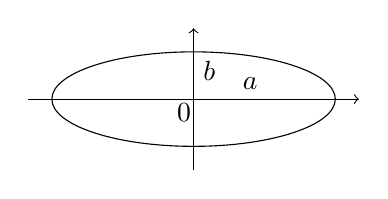
\begin{tikzpicture}[scale=0.6]
\draw (0,0) ellipse (3cm and 1cm);
\draw[->] (-3.5,0)--(3.5,0);
\draw[->] (0,-1.5)--(0,1.5);
\draw	(1.2,0) node[anchor=south] {$a$};
\draw	(0,0.6) node[anchor=west] {$b$};
\draw	(-0.2,0.1) node[anchor=north] {$0$};


\end{tikzpicture}

\end{minipage}
\hspace{0.5cm}
\begin{minipage}[b]{0.45\linewidth}

\centering
$$\frac{y^2}{b^2}+\frac{x^2}{a^2}=1$$
$$y=b\sqrt{1-\frac{x^2}{a^2}}\text{ mit }x,y>0$$

\end{minipage}
\end{figure}
$$F=4\int ^{a}_{0}b\sqrt {1-\dfrac {x^{2}}{a^{2}}}dx$$
mit $x=au$, $dx=adu$ $$F=4\int ^{1}_{0}b\sqrt {1-u^2}adu$$$$=4ab\int ^{1}_{0}\sqrt {1-u^2}du$$ mit $u=\sin t$, $du=\cos tdt$
$$4ab\int ^{\pi /2}_{0}\sqrt {1-\sin^2t}\cos t dt$$$$=4ab\int ^{\pi /2}_{0}\cos ^{2}tdt=\left.\frac{4ab}{2}\left( t+\sin t\cos t\right) \right| ^{\pi /2}_{0}$$ $$=\pi ab$$
\end{enumerate}  



\section{Integration rationaler Funktionen (Partialbruchzerlegung)}
Sei $R(x)=\frac{P(x)}{Q(x)}$ eine Rationale Funktion, d.h. $P,Q$ sind polynome mit reelen Koeffizienten. Die Partialbruchzerlegung ist eine Darstellung von $R(x)$ als summe von ``elementaren'' rationale Funktionen. Sie basiert auf einem Korollar des Fundamentales Satzes der Algebra, das sagt, dass jedes reelle Polynom ein Produkt von linearen und quadratischen Polynomen mit $\mathbb{R}$ Koeffizienten. 

\subsubsection*{Satz 6.27}
Sei $R(x)=\frac{P(x)}{Q(x)}$ eine rationale Funktion. Dann $$R(x)=P_1(x)+\sum ^{n}_{i=1}R_{i}\left( x\right) +\sum ^{m}_{j=1}S_{j}\left( x\right) $$ wobei $P_1=$ polynom $$R_{i}\left( x\right) =\dfrac {a_{i1}}{\left( x-x_{i}\right) }+\dfrac {a_{i2}}{\left( x-x_{i}\right) ^{2}}+\ldots +\dfrac {a_{ir_{i}}}{{\left( x-x_{i}\right)}^{r_i} }$$  $$S_{j}\left( x\right) =\dfrac {b_{j1}x+{d_{j1}}}{\left( \left(x-\alpha_{j}\right)^2+{\beta_{j}}^2\right) }+\dfrac {b_{j2}x+{d_{j2}}}{\left( \left(x-\alpha_{j}\right)^2+{\beta_{j}}^2\right)^2 }+\ldots +\dfrac {b_{j m_j}x+{d_{j m_j}}}{\left( \left(x-\alpha_{j}\right)^2+{\beta_{j}}^2\right)^{m_j} }$$

Die $\frac{1}{(x-a)}$, $\frac{bx+d}{\left( (x-\alpha )^2 +\beta ^2\right)^m}$ werden ``elementare rationale Funktionen'' genannt und wir wollen dafür Stammfunktionen bestimmen.

\subsubsection*{Bemerkung}

\begin{enumerate}
\item Das Polynom $P_1(x)$ tritt nur auf, falls $\deg P>\deg Q$. In diesem Fall berechnet mann $P_1(x)$ mit Polynom division und es gilt $p(x)=P_1(x)-Q(x)+P_2(x)$ mit $\deg P_2 < \deg Q$
\item Das nennerpolynom $Q(x)$ besitze
\begin{itemize}
\item Die reelen Nullstellen $x_i$ mit Vielfachheit $r_i$
\item Die Komplexe Nullstellen $z_j=\alpha _j+i\beta_j$ mit Vielfachheit $m_j$ und damit komplex Konjugierte Nullstellen $\overline{z_j}=\alpha _j-i\beta _j$
\end{itemize}
\item Unbekannte Parameter, die bestimmt werden müssen
$$a_{ik}\text{\hspace{20mm}}k=1,\dots ,r_i\text{\hspace{10mm}}i=1,\dots,n$$
$$\beta _{jl},\alpha _{jl}\text{\hspace{15mm}}l=1,\dots ,m_j\text{\hspace{10mm}}j=1,\dots,m$$
Diese Parameter werden durch Koeffizientenvergleich berechnet, die rechte Seite wird dabei auf den Hauptnenner gebracht.
\end{enumerate}
%%
\subsubsection{Beispiel}
$R(x)=\frac{1-x}{x^2(x^2+1)}$
Ansatz: $$R(x)=\frac{a_1}{x}+\frac{a_2}{x^2}+\frac{b_1x+d_1}{x^2+1}$$$$\Rightarrow 1-x=x(x^2+1)a_1+a_2(x^2+1)+x^2(b_1x+d_1)$$
Ausmultiplizieren:
$$1-x=(a_1+b_1)x^3+(a_2+d_1)x^2+a_1x+a_2$$
Koeffizientenvergleich:
$$a_1+b_1=0\text{\hspace{10mm}}a_2+d_1=0\text{\hspace{10mm}}a_1=-1\text{\hspace{10mm}}a_2=1$$
Partialbruchzerlegung:
$$\frac{1-x}{x^2(x^2+1)}=-\frac{1}{x}+\frac{1}{x^2}+\frac{x-1}{x^2+1}$$
\subsubsection*{Grundtypen der Integration rationaler Funktionen}
\begin{itemize}
\item \underline{Typ O:} Polynom:$$\int \sum a_{n}x^{n}dx=\sum a_{n}\dfrac {x^{n+1}}{n+1}+c$$
\item \underline{Typ I:} Inverse Potenzen \[\int {\frac{{dx}}{{(x - {x_0})}^r}}  = \left\{ {\begin{array}{*{20}{c}}
{\log \left| {x - {x_0}} \right| + c}&{{\text{für = 1}}}\\
{\frac{1}{{(1 - r)}}\frac{1}{{{{(x - {x_0})}^{r - 1}}}}}&{{\text{für}} \ge {\rm{2}}}
\end{array}} \right.\]

\item \underline{Typ II:}
$$\int { \dfrac {bx+d}{\left[ \left( x-\alpha \right) ^{2}+\beta ^{2}\right] ^{m}}dx}$$
Substitution: $x-\alpha =\beta t$, $dx=\beta dt$ ergibt $$\int {\dfrac {b\lbrack \beta t+\alpha\rbrack +d}{(t^2 +1)^m \beta ^{2m}} \beta dt}$$ Dies hat die allgemeine Form $$\int{\frac{ct+b}{(t^2+1)^m}dt}=c\int{\frac{t}{(t^2 +1)^m}dt}+\int{\frac{b}{(t^2 +1)^m} dt}$$
$$\int{\frac{t}{(t^2 +1)^m}dt}\text{\hspace{10mm} mit }t^2+1=u, 2t dt=du$$
$$=\frac{1}{2}\int{\frac{du}{u^m}} = \left\{ {\begin{array}{*{20}{c}}
{\frac{{{u^{ - m + 1}}}}{{2(1 - m)}}}&{{\rm{, }}m \ge 2}\\
{\frac{1}{2}\ln \left| u \right|}&{\text{, }m = 1}
\end{array}} \right. = \left\{ {\begin{array}{*{20}{c}}
{\frac{1}{{2(1 - m)}}\frac{1}{{({t^2} + 1)}}(1 - m)}&{{\rm{, }}m \ge 2}\\
{\frac{1}{2}\ln \left| {1 + {t^2}} \right|}&{\text{, }m = 1}
\end{array}} \right.$$
Sei 
$$I_m :=\int{\frac{dt}{(t^2 +1)^m}}$$
$$\text{Für $m=1$:\hspace{10mm}}I_1=\int{\frac{dt}{(t^2 +1)}}=\arctan t + C$$
$$\text{Für $m\geq1$:\hspace{10mm}}I_m:=\int{\frac{dt}{(t^2 +1)^m}}$$
Partielle Integration ergibt:
\[{I_m}: = \int {\underbrace 1_{v'} \cdot \frac{1}{{\underbrace {{{({t^2} + 1)}^m}}_u}}dt}  = \frac{t}{{{{({t^2} + 1)}^m}}} + \int {\frac{{t \cdot 2m \cdot t}}{{{{({t^2} + 1)}^{m + 1}}}}dt} \]
$$=\frac{t}{(t^2 +1)^m} + 2m\int{\frac{t^2 +1-1}{(t^2 +1)^{m+1}}dt}$$
$$\frac{t}{(t^2 +1)^m}+2m\int{\frac{1}{(t^2 +1)^m}dt}-2m\int{\frac{1}{(t^2 +1)^{m+1}}dt}$$
$$\Rightarrow I_m=\frac{t}{(t^2 +1)^m}+2m\{ I_m - I_{m+1} \}$$
woraus $$I_{m+1}=\frac{1}{2m}\left[\frac{t}{(t^2 +1)^m} + \left(\frac{2m-1}{2m}\right)I_m\right]$$
z.B.$$I_2=\int{\frac{dt}{(t^2 +1)^2}}=\frac{1}{2}\left[ \frac{t}{(t^2 +1)}+\frac{1}{2}I_1\right]$$
$$=\frac{1}{2}\left[ \frac{t}{(t^2 +1)^2}+\frac{1}{2}\arctan t\right] + C$$
\end{itemize}
\subsubsection*{Beispiel 6.28}
\begin{enumerate}
\item $$\frac{1}{x^2 -3x -4}=\frac{1}{(x-4)(x+1)}=\frac{A}{x-4}+\frac{B}{x+1}$$
$$\Rightarrow A(x+1)+B(x-4)=1$$
$$x=4\Rightarrow A\cdot 5=1\Rightarrow A=\frac{1}{5}$$
$$x=-1\Rightarrow B\cdot (-5)=1\Rightarrow B=-\frac{1}{5}$$
\[\int {\frac{1}{{{x^2} - 3x - 4}}dx = \frac{1}{5}\int {\left( {\frac{1}{{x - 4}} - \frac{1}{{x + 1}}} \right)dx = \frac{1}{5}} } \ln \left| {\frac{{x - 4}}{{x + 1}}} \right| + c\]
\item \[\frac{9}{{{x^3} - 3x - 2}} = \frac{9}{{(x - 2){{(x + 1)}^2}}} = \frac{A}{{x - 2}} + \frac{{Bx + C}}{{{{(x + 1)}^2}}}\]
\[A{(x + 1)^2} + (Bx + C)(x - 2) = 9\]

$$x=-1\Rightarrow(-B+C)(-3)=9$$
$$x=2\Rightarrow A(9)=9\Rightarrow A=1$$
$$x=0\Rightarrow A+C(-2)=9\Rightarrow -2C=8\Rightarrow C=-4$$
$$(-B+C)=-3\Rightarrow B=C+3=-1$$
$$\Rightarrow \frac{9}{x^3-3x-2}=\frac{1}{x-2}+\frac{-x-4}{(x+1)^2}$$
\[\int {\frac{9}{{{x^3} - 3x - 2}}dx = \int {\left( {\frac{1}{{x - 2}} + \frac{{ - x - 1}}{{{{(x + 1)}^2}}} - \frac{3}{{{{(x + 1)}^2}}}} \right)dx} } \]
\[ = \ln \left| {x - 2} \right| - \ln \left| {x + 1} \right| + \frac{3}{{x + 1}} + c\]
\[ = \ln \left| {\frac{{x - 2}}{{x + 1}}} \right| + \frac{3}{{x + 1}} + c\]
\end{enumerate}
\section{Das Uneigentliche Integral}
Sei $f$ eine unbeschränkte Funktion. Dann ist $f$ nicht R. Integrierbar, z.B. $\int\limits_0^1 {\frac{1}{{\sqrt x }}} dx$ hat keinen Sinn. Aber $\forall\varepsilon>0$ ist $\frac{1}{\sqrt{x}}\in\left[\varepsilon,1 \right]$ stetig also Integrierbar. Der Wert des Integral ist \[\int\limits_\varepsilon ^1 {\frac{1}{{\sqrt x }}} dx = \left. {2\sqrt x } \right|_\varepsilon ^1 = 2 - 2\sqrt \varepsilon  \] also existiert \[\mathop {\lim }\limits_{\varepsilon  \searrow 0} \int\limits_\varepsilon ^1 {\frac{1}{{\sqrt x }}} dx = 2\] Dies ist ein Beispiel von uneigentlichen R. Integral.

\begin{definition}{6.29}
Sei $f$ eine Funktion auf einem offenen Interval $(a,b)$, deren Einschränkung auf jedes kompakte Teilinterval $\lbrack a',b'\rbrack$ integrierbar ist. Dann das uneigentliche Integral von $f$ von $a$ bis $b$ definiert als \[\int\limits_a^b {f(x)dx: = \mathop {\lim }\limits_{a' \searrow a} \mathop {\lim }\limits_{b' \nearrow b} } \int\limits_{a'}^{b'} {f(x)dx} \] falls diese Grenzwerte existieren ($a$ und $b$ können $\pm \infty$ sein)
\end{definition}

 \subsubsection*{Bemerkung 6.30}
\begin{enumerate}
\item Ist $f$ schon auf $\lbrack a,b\rbrack$ definiert und integrierbar, so existiert das Uneigentliche Integral und stimmt mit dem üblichen bestimmten Integral überein.
\item Ist $f$ schon $\lbrack a,b)$ definiert und auf jedem kompakten Teilinterval der Form $\lbrack a,b'\rbrack$ integrierbar, so gilt schon  \[\int\limits_a^b {f(x)dx = \mathop {\lim }\limits_{b' \nearrow b} } \int\limits_a^b {f(x)dx} \]
\subsubsection*{Beispiel}
\[\int\limits_0^\infty  {{e^{ - x}}}  = \mathop {\lim }\limits_{b \to \infty } \int\limits_{{0}}^b {{e^{ - x}}dx}  = \lim \left( {\left. { - {e^{ - x}}} \right|_{{0}}^b} \right) = \mathop {\lim }\limits_{b \to \infty } \left( { - {e^{ - b}} + 1} \right) = 1\]
\item Vorsicht: Die beiden Grenzwerte müssen im allgemeinen unabhängig voneinander genommen werden. 
\subsubsection*{Beispiel}
\[\int\limits_{ - b}^b {xdx = 0} \text{\hspace{10mm}}\forall b>0\text{, und daher}\]
\[\mathop {\lim }\limits_{b \to \infty } \int\limits_{ - b}^b {xdx = \lim \left( {\frac{{{b^2}}}{2} - \frac{{{b^2}}}{2}} \right) = \mathop {\lim }\limits_{b \to \infty } 0 = 0} \]
Die einzelnen Grenzwerte von $\int\limits_a^b {xdx} $ für $b\rightarrow \infty$ und $a\rightarrow -\infty$ existieren dagegen nicht \[\left( {\int\limits_a^b {xdx = \left. {\frac{{{x^2}}}{2}} \right|_a^b = \frac{{{b^2}}}{2} - \frac{{{a^2}}}{2}} } \right)\] und somit auch nicht das uneigentliche Integral $\int\limits_{ - \infty }^\infty  {xdx} $
\item Alle Grundeigenschaften und Integrationstechniken für das bestimmte Integral gelten ebenso für das uneigentliche Integral. 
\end{enumerate}
Als Beispiel beweisen wir folgendes nützliches Konvergenzkriterium für Reihen
\subsubsection*{Satz 6.30}
Sei $f:\lbrack 1,\infty )\rightarrow \mathbb{R}_+$ monoton fallend. Dann konvergiert $\sum\limits_{k = 1}^\infty  {f(k)}$ genau dann wann $\int\limits_1^\infty  {f(x)dx} $ existiert. In diesem Fall gilt: \[0 \le \sum\limits_{k = 1}^\infty  {f(k)}  - \int\limits_1^\infty  {f(x)dx}  \le f(1)\]
\subsubsection*{Beweis}
\begin{center}
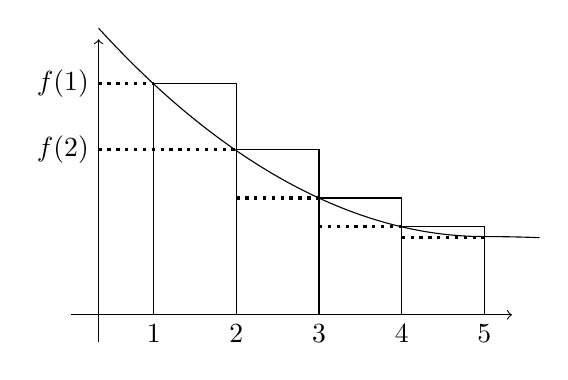
\begin{tikzpicture}[scale=0.7]
% horizontal axis
\draw[->] (-0.5,0) -- (7.5,0) node[anchor=north] {};
% labels
\draw	(1,0) node[anchor=north] {1}
		(2.5,0) node[anchor=north] {2}
		(4,0) node[anchor=north] {3}
		(5.5,0) node[anchor=north] {4}
		(7,0) node[anchor=north] {5}
		(0,3) node[anchor=east] {$f(2)$}
		(0,4.2) node[anchor=east] {$f(1)$};
		

% vertical axis
\draw[->] (0,-0.5) -- (0,5) node[anchor=east] {};
% 3 columns
\draw (1,0)--(1,4.2)--(2.5,4.2)--(2.5,3);
\draw (2.5,0)--(2.5,3)--(4,3);
\draw (4,0)--(4,3);
\draw (4,2.12)--(5.5,2.12);
\draw (5.5,2.12)--(5.5,1.6);
\draw (5.5,0)--(5.5,1.6)--(7,1.6)--(7,0);

\draw (0,5.2) parabola bend (7,1.42)(8,1.4);

\draw[dotted, very thick](0,4.2)--(1,4.2)
[dotted, very thick](0,3)--(2.5,3)
[dotted, very thick](2.5,2.12)--(4,2.12)
[dotted, very thick](4,1.6)--(5.5,1.6)
[dotted, very thick](5.5,1.4)--(7,1.4);

\end{tikzpicture}
\end{center}


$$f(1) + f(2) +  \ldots  + f(n - 1) \ge \int\limits_1^n {f(x)dx \ge f(2) +  \ldots f(n)} $$
$$\sum\limits_{k = 1}^n {f(k) - f(n)}  = \sum\limits_{k = 1}^{n - 1} {f(x) \ge \int\limits_1^n {f(x)dx \ge \sum\limits_{k = 1}^{n - 1} {f(k + 1) = } \sum\limits_{k = 1}^n {f(x) - f(1)} } } $$
$$\sum\limits_{k = 1}^n {f(k) - f(n) \ge \int\limits_1^n {f(x)dx \ge \sum\limits_{k = 1}^n {f(k) - f(1)} } } \text{\hspace{10mm}(\textasteriskcentered)} $$
 $$\Rightarrow 0<f(n) \le \sum\limits_{k = 1}^n {f(k) - \int\limits_1^n {f(x)dx \le f(1)} } $$
Aus \[\sum\limits_{k = 1}^{n - 1} {f(k) \ge \int\limits_1^n {f(x)dx} } \] folgt das, \[\sum\limits_{k = 1}^\infty  {f(k) < \infty  \Rightarrow \int\limits_1^\infty  {f(x)dx < \infty } } \] und, aus \[\int\limits_1^n {f(x)dx \ge \sum\limits_{k = 1}^{n - 1} {f(k + 1)} } \] folgt dass \[\int\limits_1^\infty  {f(x)dx < \infty  \Rightarrow \sum\limits_{k = 1}^\infty  {f(k) < \infty } } \]
Aus (\textasteriskcentered) folgt: \[0<f(n) \le \sum\limits_{k = 1}^\infty  {f(k)}  - \int\limits_1^\infty  {f(x)dx \le f(1)} \]

\subsubsection*{Beispiel 6.31}%Page 68, top
\begin{enumerate}
\item $\sum {(s) = \sum\limits_{k = 1}^\infty  {\frac{1}{{{k^s}}}} } $ existiert für alle $s>1$ 
$$\int\limits_1^\infty  {\frac{1}{{{x^s}}}dx}  = \mathop {\lim }\limits_{b \to \infty } \int\limits_1^b {{x^{ - s}}dx}  = \lim \left\{ {\begin{array}{*{20}{c}}
{\log \left| b \right|}&{s = 1}\\
{\left. {\frac{{{x^{ - s + 1}}}}{{1 - s}}} \right|_1^b}&{s > 1}
\end{array}} \right. $$$$= \left\{ {\begin{array}{*{20}{c}}
{\text{divergent falls }s = 1}\\
{\text{konvergent gegen }\frac{1}{{s - 1}}}
\end{array}} \right.$$
und
$$0 \le \sum\limits_{n = 1}^\infty  {{n^{ - s}}}  - \int\limits_1^\infty  {f(x)dx}  \le f(1) = 1$$$$ \Rightarrow \frac{1}{{s - 1}}\sum\limits_{n = 1}^\infty  {{n^{ - s}}}  \le 1 + \frac{1}{{s - 1}} = \frac{s}{{s - 1}}$$
\item \[\int\limits_{ - \infty }^\infty  {\left| x \right|{e^{ - {x^2}}}dx}  =  - \int\limits_{ - \infty }^0 {x{e^{ - {x^2}}}dx}  + \int\limits_0^\infty  {x{e^{ - {x^2}}}dx}  = 2\int\limits_0^\infty  {x{e^{ - {x^2}}}dx} \]
\[\int\limits_0^b {x{e^{ - {x^2}}}dx = \frac{1}{2}\int\limits_0^{{b^2}} {{e^{ - u}}du} }\text{\hspace{10mm} mit }u=x^2, du=2xdx \]
\[ = \frac{1}{2}\left( {1 - {e^{ - {b^2}}}} \right) \to \frac{1}{2}\text{ für }b\rightarrow \infty\]
Somit gilt \[\int\limits_{ - \infty }^\infty  {\left| x \right|{e^{ - {x^2}}}dx = 1} \]
\item Wir haben die folgende einfache aber wichtige Beispiele
\begin{enumerate}
\item \[\int\limits_{ a }^\infty  {\frac{{dx}}{{{x^s}}}}  = \left\{ {\begin{array}{*{20}{c}}
{\begin{array}{*{20}{c}}
{\frac{{{a^{1 - s}}}}{{s - 1}}}&\text{für}&{s > 1}
\end{array}}\\
{\begin{array}{*{20}{c}}
\infty &{{\text{für}}}&{s \le 1}
\end{array}}
\end{array}} \right.\]

\item Für alle $a<b$ und $s\in\mathbb{R}$ gilt \[\int\limits_a^b {\frac{{dx}}{{{{(x - a)}^s}}}}  = \left\{ {\begin{array}{*{20}{c}}
{\begin{array}{*{20}{c}}
{\frac{{{{(b - a)}^{1 - s}}}}{{1 - s}}}&\text{für}&{s < 1}
\end{array}}\\
{\begin{array}{*{20}{c}}
\infty &{{\text{für}}}&{s \ge 1}
\end{array}}
\end{array}} \right.\]
\end{enumerate}
\end{enumerate}
\subsubsection*{Satz 6.32 (Majorantenkriterium)}
\begin{enumerate}[\indent a)]
\item Sei $f:\lbrack a,\infty )\rightarrow\mathbb{R}$ stetig. Dann gilt $$\forall x:\left| f(x)\right| <g(x)$$ und $\int\limits_a^\infty  {g(x)}$ konvergent $\Rightarrow \int {f(x)dx} $ (absolut) konvergent.
\item Weiterhin gilt folgende Umkehrung: $\forall x:0\leq g(x)\leq f(x)$ und $\int\limits_a^\infty  {g(x)}$ divergent $\Rightarrow \int\limits_a^\infty  {f(x)}$ divergent.
\end{enumerate}

\subsubsection*{Beispiel 6.33}
\begin{enumerate}
\item \[\int\limits_0^\infty  {\frac{{{t^2}}}{{{{\left( {1 + 6{t^2}} \right)}^{5/3}}}}dt}  < \int\limits_0^\infty  {\frac{{{t^2}}}{{{{\left( {6{t^2}} \right)}^{5/3}}}}dt}  < \int {\frac{c}{{{t^{4/3}}}}dt < \infty } \]
$$\Rightarrow\int\limits_0^\infty  {\frac{{{t^2}}}{{{{\left( {1 + 6{t^2}} \right)}^{5/2}}}}dt} \text{ konvergiert}$$
\item \[\int\limits_0^\infty  {\frac{{{t^2}}}{{{{\left( {1 + 6{t^2}} \right)}^{3/2}}}}dt} \]   
\[\frac{{{t^2}}}{{{{\left( {1 + 6{t^2}} \right)}^{3/2}}}} > \frac{{{t^2}}}{{{{\left( {12{t^2}} \right)}^{3/2}}}} > \frac{c}{t}\text{\hspace{10mm}}t\geq 1\]
\[\Rightarrow\int\limits_0^\infty  {\frac{{{t^2}}}{{{{\left( {1 + 6{t^2}} \right)}^{5/2}}}}} dt\text{ divergiert weil }\int\limits_0^\infty  {\frac{c}{t}} dt\text{ divergiert}\]
\item Exponentialintegral:
\[{E_i}(x): = \int\limits_{ - \infty }^x  {\frac{{{e^t}}}{t}dt} \text{ für }x<0\]
Da $\mathop {\lim }\limits_{t \to  - \infty } t{e^t} = 0$, gibt es $c>0$ mit $\left| {t{e^t}} \right| \le c$, $\forall t\in\lbrack -\infty ,x\rbrack$, und somit gilt \[\left| {\frac{{{e^t}}}{t}} \right| = \left| {\frac{{t{e^t}}}{{{t^2}}}} \right| \le \frac{c}{{{t^2}}}\] Mit der Konvergenz des Integrals $\int\limits_{ - \infty }^x {\frac{1}{{{t^2}}}dt} $ folgt die (Absolut) Konvergenz des $E_i(x)$ für alle $x<0$
\end{enumerate}